%% Template for a preprint Letter or Article for submission
%% to the journal Nature.
%% Written by Peter Czoschke, 26 February 2004
%%

\documentclass{nature}
%\documentclass[12pt]{article}

%% make sure you have the nature.cls and naturemag.bst files where
%% LaTeX can find them

\bibliographystyle{naturemag}

\usepackage{graphicx}
\usepackage{amssymb,amsfonts,amsmath}
\usepackage{subfigure}
\usepackage{stfloats}


%% OPTIONAL MACRO DEFINITIONS
\def\s{\sigma}
\newcommand{\be}[0]{\begin{equation}}
\newcommand{\ee}[0]{\end{equation}}
\newcommand{\lb}[0]{\left(}
\newcommand{\rb}[0]{\right)}


%\title{Inefficacy of stratospheric sulfate aerosol injections for saving the West Antarctic Ice Sheet} % 94chars
%\title{Inefficacy of geoengineering by stratospheric aerosols for saving the West Antarctic Ice Sheet} 
%\title{Geoengineering by stratospheric sulfate aerosols cannot save the West Antarctic Ice Sheet} % 89
\title{Stratospheric sulfate aerosol injections cannot preserve the West Antarctic Ice Sheet} % 81
%\title{Ineffective preservation of the West Antarctic Ice Sheet under stratospheric sulfate aerosol injections}

%% Notice placement of commas and superscripts and use of &
%% in the author list


\author{K. E. McCusker*$^{1,2}$, \& D. S. Battisti,$^{2}$, \& C. M. Bitz$^2$}

% NatGeo requirements:
% Title If possible, the title should give a sense of the main new finding, and should not exceed 90 characters, including spaces. Nature Geoscience titles do not contain technical terms or abbreviations unless absolutely necessary. We strongly discourage punctuation or active verbs.@@
% Letter 2,000 words no methods, 3 figures
% Article 3,000 words no methods, include section titles, 6 figures. No refs in abstract. ~500 words of Intro. 1-2 para of conclusions


\begin{document}

\maketitle

\begin{affiliations}
 \item Department of Atmospheric Sciences, University of Washington, Seattle, WA 98195, USA
 \item School of Earth and Ocean Sciences, University of Victoria, Victoria, BC, V8V 1B5, Canada
\end{affiliations}


\begin{abstract}

%Solar radiation management (SRM) via injection of sulfate aerosols into the stratosphere has garnered attention for its potential to reduce the climate impacts of global warming, including sea level rise (SLR) \cite{moore10,irvine12}. However, the dynamical influences on SLR that arise from offsetting increases in tropospheric greenhouse gases with stratospheric sulfate aerosols \cite{ammann10} have not previously been considered. The West Antarctic Ice Sheet is particularly vulnerable as Southern Ocean warming lingers at depth indefinitely \cite{gillett11}. Here we use a fully-coupled global climate model (GCM) to investigate whether rapidly increasing stratospheric sulfate aerosol concentrations after a period of global warming could reverse steric sea level rise and preserve Antarctic ice sheets by cooling subsurface ocean temperatures. We contrast this SRM method with an alternative climate management strategy in which all greenhouse gases (GHG) are returned to preindustrial levels. We find that the rapid addition of a stratospheric aerosol layer does not effectively counteract surface and upper level atmospheric circulation changes caused by increasing greenhouse gases. As a result, SRM does not effectively prevent upwelling of warm subsurface water to within contact with the ice shelves. Even in the absence of atmospheric warming, basal melt due to ocean circulation changes under sulfate aerosol SRM risks destabilizing West Antarctica. By contrast, removal of atmospheric greenhouse gases restores the wind stress on the ocean, yielding relatively cooler subsurface ocean temperatures and protecting West Antarctica. 
Solar radiation management (SRM) via injection of sulfate aerosols into the stratosphere has the potential to reduce the climate impacts of global warming, including sea level rise (SLR). However, changes in atmospheric and oceanic circulation that can significantly influence the rate of melting at the base of Antarctic marine ice shelves and the associated SLR have not previously been considered. Here we use a fully-coupled global climate model (GCM) to investigate whether rapidly increasing stratospheric sulfate aerosol concentrations after a period of global warming could preserve Antarctic ice sheets by cooling subsurface ocean temperatures. We contrast this SRM method with an alternative strategy in which all greenhouse gases (GHG) are returned to preindustrial levels. We find that the rapid addition of a stratospheric aerosol layer does not effectively counteract surface and upper level atmospheric circulation changes caused by increasing GHGs, resulting in continued upwelling of warm water in proximity of ice shelves, especially in the vicinity of the already unstable Pine Island Glacier in West Antarctica. Even in the absence of atmospheric warming, basal melt due to ocean circulation changes under sulfate aerosol SRM risks destabilizing West Antarctica. By contrast, removal of GHGs restores the circulation, yielding relatively cooler subsurface ocean temperatures to better preserve West Antarctica. %209 words

%The West Antarctic Ice Sheet is particularly vulnerable as Southern Ocean warming lingers at depth indefinitely \cite{gillett11}. Here we use a fully-coupled global climate model (GCM) to investigate whether rapidly increasing stratospheric sulfate aerosol concentrations after a period of global warming could reverse steric sea level rise and preserve Antarctic ice sheets by cooling subsurface ocean temperatures. We contrast this SRM method with an alternative climate management strategy in which all greenhouse gases (GHG) are returned to preindustrial levels. We find that the rapid addition of a stratospheric aerosol layer does not effectively counteract surface and upper level atmospheric circulation changes caused by increasing greenhouse gases. As a result, SRM does not effectively prevent upwelling of warm subsurface water to within contact with the ice shelves. Even in the absence of atmospheric warming, basal melt due to ocean circulation changes under sulfate aerosol SRM risks destabilizing West Antarctica. By contrast, removal of atmospheric greenhouse gases restores the wind stress on the ocean, yielding relatively cooler subsurface ocean temperatures and protecting West Antarctica.  %melting at the base of Antarctic marine ice shelves, which has the potential to contribute substantially to SLR and is highly sensitive to changes in atmospheric and oceanic circulation, has not previously been considered.

\end{abstract}

The retreat of the Pine Island and Thwaites Glaciers has accelerated, with a rapid collapse of the West Antarctic ice sheet (WAIS) possible within as little as a few centuries \cite{joughin14,rignot14,favier14}. The mass contribution to sea level rise (SLR) from such a collapse is thought to compare with or even exceed projected steric SLR \cite{church13}. Given that the retreat of Pine Island and Thwaites Glaciers may be slowed or reversed if basal melt rates are decreased \cite{favier14}, an important question is whether solar radiation management (SRM) may be able to delay or even prevent a WAIS collapse, as has been suggested \cite{blackstock09}.

A large amount of mass loss from ice sheets occurs due to basal melt of the ice shelves \cite{joughin11}, the floating extensions of land ice sheets. In West Antarctica, the face of these ice shelves extend from the surface to several hundred meters depth, near the level of the Circumpolar Deep Water (CDW), a subsurface water mass that is slightly warmer (-1$^\circ$C to 1$^\circ$C; \cite{yin11}) than waters above and below it. An increase in the temperature of CDW or in the rate that CDW is brought onto the continental shelf due to regional wind variability can greatly increase basal melting of ice shelves \cite{thoma08,joughin11}, causing ice shelf thinning and a subsequent reduction in the buttressing stress, which leads to an increase in ice stream velocity and ice mass loss\cite{oppenheimer98,pritchard12}. Thus, ice shelf disintegration can happen even in the absence of large atmospheric warming \cite{oppenheimer98}. %@@colin suggests I get an updated ref. Try depoorter Nature 2013 (have to get and read). Or Dupont & Alley GRL 2005.  %In short, a small warming of CDW, or a greater propensity for CDW to encroach on continental shelves, has the potential to cause ice shelf disintegration even in the absence of large atmospheric warming \cite{oppenheimer98}. 

SRM has been shown to reduce the rate of global mean sea level rise by examining observed relationships between the response of sea level to volcanic eruptions \cite{moore10}, which temporarily lower sea level by briefly reducing ocean heat content \cite{church05,gleckler06}, and by examining the steric height changes in an intermediate complexity climate model \cite{irvine12}. Irvine et al. (2012) additionally include the contribution to sea level from mass input with a scaling to the global mean surface temperature anomaly. However, changes in oceanic circulation that can have significant impacts on basal melting of ice shelves \cite{steig13,joughin11,thoma08} have not previously been considered.
%Curbing sea level rise via SRM has been explored using observed relationships between the response of sea level to volcanic eruptions \cite{moore10}, which temporarily lower sea level by briefly reducing ocean heat content \cite{church05,gleckler06}, and by examining the steric height changes in an intermediate complexity climate model \cite{irvine12}; Irvine et al. (2012) additionally include the contribution to sea level from mass input with a scaling to the global mean surface temperature anomaly. These studies find that SRM would reduce the rate of global mean sea level rise. However, changes in oceanic circulation, which can have significant impacts on basal melting of ice sheets and shelves \cite{steig13,joughin11,thoma08} have not previously been considered. 

The subsurface Southern Ocean temperature structure is strongly influenced by the surface wind stress \cite{fyfe07,spence14}, which in turn is set by the circumpolar westerly jet. McCusker et al. (2012) showed in a set of idealized simulations that when climate is stabilized using a stratospheric sulfate layer that counteracts growing CO$_2$ concentrations, an anomalous poleward-intensified zonal wind stress on the Southern Ocean remains that causes upwelling of warmer subsurface waters to the level of ice sheet outlets. Warmed subsurface ocean waters that destabilize marine ice sheets may introduce threshold behavior \cite{notz09} or become nonlinear with increased warming \cite{joughin14}.

To promptly avoid SLR in the face of rising greenhouse gases (GHGs), a large, rapid shock of stratospheric aerosols would need to be deployed to reverse heat uptake by the ocean. Any delays in implementation would allow additional ocean heat storage that may linger at intermediate depths for centuries \cite{gillett11}. SRM is most likely to be deployed only after a period of global warming that is deemed to be unacceptably large. Could a subsequent implementation of sulfate SRM preserve Antarctic ice sheets? Here we investigate with the Community Climate System, version 4 (CCSM4) the impact of a rapidly increased stratospheric sulfate aerosol burden on atmospheric and oceanic circulation in proximity of Antarctica. We contrast these results with an alternative management scenario in which GHGs are abruptly returned to preindustrial levels --- the ultimate, if not impractical, climate engineering.  %590 words

\section{Sea level rise and atmospheric circulation}

Density changes in our scenarios constitute the `steric' contribution to sea level rise (Methods). However, as CCSM4 (and most models of its class) lacks dynamical ice sheet behavior, and ice shelves and ice shelf cavities are absent, the contribution of mass input from the WAIS and other Antarctic ice sheets cannot be explicitly calculated. We instead focus on the large-scale oceanic temperature anomalies that determine melt rates near the ice shelves. 

The time evolution of global mean surface air temperature (SAT) for business-as-usual (RCP8.5) and climate engineering scenarios is shown in Figure \ref{fig:gmts}a. Sulf (blue) represents a scenario in which drastic climate engineering is required to stop sea levels from further rising, and hence entails a quick and large decrease in net radiative forcing via a rapid increase in stratospheric aerosol burden. This decrease in radiative forcing avoids a large amount of warming compared to business-as-usual (Figure \ref{fig:gmts}a; RCP8.5 in red). The global and annual mean SAT linear trend for the first decade following the start of SRM (years 2036-2045) is -0.94$^\circ$C/decade for the ensemble mean, and the land-only trend is even greater at -1.2 $^\circ$C/decade. As such, Sulf returns global mean SAT to roughly the end of the 20th century average (1970-1999) by the following decade (2045-2054; SAT anomaly of -0.03$^\circ$C) and is much cooler than RCP8.5, which is 1.83$^\circ$C warmer than the end of the 20th century at that time. A second climate engineering scenario consisting of an instantaneous removal of GHGs to preindustrial conditions (GHGrem in green) gives a change in SAT that is broadly equivalent to that of Sulf for the same time period (-0.36$^\circ$C).

Global average sea level due to changes in ocean density, in isolation of possible mass change from dynamical ice-loss or exceptional melt (i.e., melt beyond 1 m of snow water equivalent; see Methods), reverses course and starts declining upon initiation of climate engineering (Figure \ref{fig:gmts}b). Nearly 30 cm of steric sea level rise is avoided by century's end when a sulfate layer is implemented, consistent with previous findings \cite{irvine12}. Thus, a high rate of sulfate injection could promptly reduce or avoid a substantial amount of steric sea level rise, at the expense of potentially hazardous, large SAT trends. Removal of GHGs is equally effective at decreasing sea level. Next we consider whether changes in the distribution of ocean temperature might be poised to cause greater basal melt to marine ice shelves. 

Numerical simulations of SRM with stratospheric aerosols have shown residual SH poleward intensified winds induced by differences in the vertical temperature structure of a stratospheric sulfate layer versus well-mixed tropospheric carbon dioxide \cite{ammann10,mccusker12}. These temperature anomalies and corresponding upper atmosphere and surface wind changes share features with those induced by ozone depletion \cite{gillett03,gillett13,sigmond11,thompson11} and increasing greenhouse gases \cite{gillett13,sigmond11,polvani11}. Although mechanisms and structural details differ somewhat depending on the type of upper atmospheric forcing, the fundamental cause is the same: zonal wind shear is modified via thermal wind balance altered by an anomalous increase in the stratospheric pole-to-equator temperature gradient. Strengthened SH lower stratospheric/upper tropospheric winds are then associated with increased eastward eddy propagation, which in turn shifts the critical latitude for Rossby wave breaking poleward, leading to poleward shifted surface westerlies \cite{chen07}.

When aerosols are quickly increased in the stratosphere, large temperature anomalies are generated in the upper troposphere and stratosphere (Figure \ref{fig:vert}a). The zonal mean temperature structure with height is a combination of strong tropical lower stratospheric heating due to aerosols \cite{ferraro11} and high latitude stratospheric cooling due to GHGs, with little change in the lower tropospheric temperature. The resultant zonal winds show a strengthened SH polar vortex and slight weakening of the subtropical jet (Figure \ref{fig:vert}b). 

The upper atmospheric deviations result in surface wind and wind stress anomalies in the SH that are comparable to those in the RCP8.5 business-as-usual scenario: they are poleward-shifted and intensified and have similar magnitudes (Figures \ref{fig:shmaps}d, \ref{fig:shmaps}e, and \ref{fig:zmtautemp}a). In contrast, when GHGs are removed from the atmosphere, the surface wind stress is very nearly returned to 20thC values (Figure \ref{fig:shmaps}f and \ref{fig:zmtautemp}a). Additionally, while both climate engineering strategies cause the sea ice edge to recover to the 20thC position (20thC and climate engineering simulations show co-located 15\% concentration contours in Figure \ref{fig:shmaps}e-f), annual average sea ice concentration near sea ice margins remains lower by up to 15\% in Sulf, but are increased beyond 20thC concentrations by almost 10\% in GHGrem (Supplementary Figure 1). The residual sea ice concentration anomalies in Sulf and GHGrem are echoed in the residual temperature anomalies shown in Figure \ref{fig:shmaps}: Figure \ref{fig:shmaps}b shows a weak local warming accompanying the reduced sea ice concentration in Sulf, while Figure \ref{fig:shmaps}c shows weak local cooling where there are small increases in sea ice concentration in GHGrem. 

\section{Implications for Antarctic ice sheets}

Both climate engineering scenarios presented here in Sulf and GHGrem greatly reduce the surface warming over Antarctica that is seen in the RCP8.5 scenario --- greater than 100\% in the case of GHGrem (compare Figure \ref{fig:shmaps}b and \ref{fig:shmaps}c with \ref{fig:shmaps}a) --- but the ocean heat uptake that occurred over the first third of the 21st century before climate engineering was initiated also poses a threat to Antarctic ice sheets, particularly the WAIS, whose grounding line is below sea level \cite{joughin11} and retreating \cite{rignot14}. % supp Fig 2 for ocean heat uptake time series?

Small ocean temperature perturbations can have a significant impact on basal melting of ice shelves; a warming of just 0.1$^\circ$C can thin 1 m of ice shelf in a year \cite{rignot02}. Zonally averaged Southern Ocean temperature anomalies in Sulf indicate that temperatures encroaching on the ice shelves average 0.15-0.20$^\circ$C warmer than 20thC (Figure \ref{fig:zmtautemp}c). Drastic reduction of greenhouse gases, however, shows zonal mean temperature near the level of ice shelves is up to 0.25$^\circ$C cooler than in Sulf (Figure \ref{fig:zmtautemp}d). The ice sheet region in Antarctica most at-risk from basal melt is the Amundsen Sea Embayment sector including Pine Island Glacier (PIG). Critically, this region reveals an even greater potential for melting under sulfate climate engineering than in the zonal average: the Sulf ensemble features an anomalous residual warming of 0.5$^\circ$C in the 200-500m layer (Figure \ref{fig:pigtemp}a). Extrapolating from Ref. 29, this temperature anomaly represents a basal melt rate of 5 m/year above the 20thC average. In contrast, removal of GHGs is effective at cooling the subsurface ocean up to 0.5$^\circ$C. %@@ Extrapolating from Ref. 27, this implies a basal melt rate of 1.5-2.0 m/yr under Sulf, maintained for 10 years. The consequence would be @@@ %Converting this 0.25$^\circ$C difference in ocean temperature between the two scenarios into a gross estimate of basal melt rate using the relationship from Ref. 27 implies that the zonal average basal melt rate in Sulf would be 2.5 m/year greater than in GHGrem. %In fact, the basal melt rate in GHGrem may even decrease beyond the rate found in the 20thC 1970-99 average, as evidenced by cooling to about 400 meters in Figure \ref{fig:zmtautemp}d. %, which is already a few tenths of a degree warmer than simulated preindustrial conditions (not shown)

GHG removal is a more effective means for cooling subsurface ocean temperatures than stratospheric aerosol injection fundamentally because of changes in circulation. The anomalous mid-depth zonal average warmth evident south of about 65$^\circ$S and between 200-400m depth in Sulf (Figure \ref{fig:zmtautemp}c) can be understood as anomalous upwelling of relatively warm CDW. This upwelling is caused by increased Ekman pumping that originates from the previously discussed poleward-intensified zonal winds (Figures \ref{fig:shmaps}e) caused by stratospheric aerosols, greenhouse gases \cite{fyfe07}, and their combination here (Figure \ref{fig:zmtautemp}a). Engineering by sulfate aerosols features anomalous upwelling poleward of 60$^\circ$S and downwelling equatorward of 60$^\circ$S -- just as in the RCP8.5 scenario (albeit with slightly smaller upwelling than in RCP8.5). In contrast, the removal of GHGs causes a reversal of sign in the zonal wind stress and wind stress curl anomalies compared to the anomalies associated with RCP8.5, resulting in weak anomalous downwelling south of 60$^\circ$S (Figure \ref{fig:zmtautemp}b), which results in the cooling of the 200-400m layer past the 20th century mean (Figure \ref{fig:zmtautemp}d). 

In the PIG region, the primary driver of the contrasting behavior between geoengineering methods is again differences in circulation. Vertical velocity responses of opposing signs (Figure \ref{fig:pigtemp}c) act on a temperature gradient that features an increase in temperature with increasing depth in these layers (Figure \ref{fig:pigtemp}d). The result is that vertical temperature advection warms the water column under sulfate engineering whereas removal of GHGs causes a cooling, which is primarily due to the Eulerian component of vertical advection (Figure \ref{fig:pigtemp}e). The mid-depth residual warming resembles the `slow timescale' response to an increase in ozone forcing wherein Southern Ocean circulation adjusts to changes in atmospheric winds and causes ocean warming from below that overcomes initial SST cooling and sea ice growth on the time scale of decades. %@@something about winds and observed warming@@%found in the zonal average and in the PIG region is a familiar response to wind forcing on the Southern Ocean that may already be increasing basal melt of Antarctic glaciers (@@cite). For example, the feature %Thus, the inability of sulfate engineering to mitigate wind anomalies caused by increased greenhouse gases yields the method unable to counteract ocean warming near ice shelves. Indeed, t
%While our GCM is not the appropriate tool to convert these temperature anomalies into a mass contribution to sea level rise, the fact remains that 
%The ice sheet region in Antarctica most at-risk from basal melt is the Amundsen Sea Embayment sector including Pine Island Glacier (PIG). This region reveals an even greater potential for melting under sulfate climate engineering than in the zonal average: the Sulf ensemble features an anomalous residual warming of 0.5$^\circ$C in the 200-500m layer (Figure \ref{fig:pigtemp}a). In contrast, removal of GHGs is effective at cooling the subsurface ocean up to 0.5$^\circ$C, a differential of 1$^\circ$C or, extrapolating from Ref. 27, a basal melt rate difference of 10m/year between the two climate engineering methods. [@@implication - use reference]. The primary driver of this contrasting behavior is again differences in circulation. Vertical velocity responses of opposing signs (Figure \ref{fig:pigtemp}d) act on a temperature gradient that features an increase in temperature with increasing depth in these layers (Figure \ref{fig:pigtemp}e). The result is that vertical temperature advection warms the water column under sulfate engineering whereas removal of GHGs causes a cooling, which is primarily due to the Eulerian component of vertical advection (Figure \ref{fig:pigtemp}c). %There is an increase in temperature due to vertical advection throughout the water column under sulfate engineering (negative values) whereas removal of GHGs causes a decrease (due to the Eulerian component). The primary driver of these disparate tendency profiles is a vertical velocity ($w$) response of opposing signs (Figure \ref{fig:pigtemp}d), primarily Eulerian, acting on a temperature gradient that features an increase in temperature with increasing depth in these layers (Figure \ref{fig:pigtemp}e). %Eulerian, eddy, and total components of the vertical advection tendency (in units of W/m$^2$) averaged from 65-74$^\circ$S are shown with depth in Figure \ref{fig:pigtemp}c. #@@re: implication: note that pritchard paper talks about thinning (m/yr) and that IS basal melt they determine. they don't speak about SLR but reread to see if can compare my numbers to theirs.

Finally, although not germane to the stability of Antarctic ice sheets, it is interesting to note the disparate temperature profiles equatorward of 60$^\circ$S between Sulf and GHGrem as well. The warming evident equatorward of 60$^\circ$S at all depths in Sulf is a combination of residual warmth from before geoengineering began, a poleward shift (fundamentally due to the atmospheric jet shift) of the nearly vertical isotherms there, and increased downwelling of warmer surface waters. This feature is noticeably absent when GHGs are instead removed from the atmosphere because the jet rapidly returns to the 20thC position, resulting in weak upwelling anomalies equatorward of 60$^\circ$S. Thus the warming equatorward of ~60$^\circ$S is also due to the changes in the atmospheric winds due to the net forcing of increased GHGs and sulfate aerosols. %resembling the 'slow timescale' response to an increase in ozone forcing described in Ref. 28, wherein Southern Ocean circulation adjusts to changes in atmospheric winds and causes ocean warming from below that overcomes initial SST cooling and sea ice growth on the time scale of decades. %Here, engineering by sulfate aerosols features anomalous upwelling poleward of 60$^\circ$S and downwelling equatorward of 60$^\circ$S -- just as in the RCP8.5 scenario (albeit with slightly smaller upwelling than in RCP8.5). In contrast, the removal of GHGs causes a reversal of sign in the zonal wind stress and wind stress curl anomalies compared to the anomalies associated with RCP8.5, resulting in weak anomalous downwelling south of 60$^\circ$S (Figure \ref{fig:zmtautemp}b), which results in the cooling of the 200-400m layer past the 20th century mean (Figure \ref{fig:zmtautemp}d). %Although not germane to the stability of Antarctic ice sheets, it is interesting to note the disparate temperature profiles equatorward of 60$^\circ$S between Sulf and GHGrem as well. The warming evident equatorward of 60$^\circ$S at all depths in Sulf is a combination of residual warmth from before geoengineering began, a poleward shift (fundamentally due to the atmospheric jet shift) of the nearly vertical isotherms there, and increased downwelling of warmer surface waters. This feature is noticeably absent when GHGs are instead removed from the atmosphere because the jet rapidly returns to the 20thC position, resulting in weak upwelling anomalies equatorward of 60$^\circ$S. Thus the warming equatorward of ~60$^\circ$S is also due to the changes in the atmospheric winds due to the net forcing of increased GHGs and sulfate aerosols.

%These results show that in the zonal mean, the Southern Ocean remains conducive to basal melting of ice shelves when stratospheric sulfate injections are implemented, but not when GHGs are removed. Examining the most at-risk ice sheet region in Antarctica, the Amundsen Sea Embayment sector including Pine Island Glacier (PIG), reveals an even greater potential for melting under sulfate climate engineering than in the zonal average: the Sulf ensemble features an anomalous residual warming of 0.5$^\circ$C in the 200-500m layer (Figure \ref{fig:pigtemp}a). In contrast, removal of GHGs is effective at cooling the subsurface ocean up to 0.5$^\circ$C, a differential of 1$^\circ$C or a basal melt rate difference of 10m/year between the two climate engineering methods. Eulerian, eddy, and total components of the vertical advection tendency (in units of W/m$^2$) averaged from 65-74$^\circ$S are shown with depth in Figure \ref{fig:pigtemp}c. There is an increase in temperature due to vertical advection throughout the water column under sulfate engineering (negative values) whereas removal of GHGs causes a decrease (due to the Eulerian component). The primary driver of these disparate tendency profiles is a vertical velocity ($w$) response of opposing signs (Figure \ref{fig:pigtemp}d), primarily Eulerian, acting on a temperature gradient that features an increase in temperature with increasing depth in these layers (Figure \ref{fig:pigtemp}e). 

\section{Discussion}

SRM using stratospheric aerosols has been suggested as a `backstop' measure that could be rapidly deployed to avoid so-called climate emergencies, one of which is the destabilization of marine ice sheets \cite{blackstock09}. However, our results indicate that it would be ineffective for this purpose. The rapid addition of stratospheric sulfate aerosols may quickly reverse steric sea level rise at the expense of deleterious land SAT trends, however circulation changes over and in the Southern Ocean are not counteracted. The result is a large-scale oceanic environment that would be favorable for further thinning of Antarctic ice shelves through basal melt, particularly in the region encompassing Antarctica's largest contributor to sea level rise \cite{shepherd12}: the already unstable Pine Island Glacier outlet \cite{rignot14}. Moreover, because these circulation changes are due to modification of the stratospheric meridional temperature gradient through the combination of sulfate aerosol deployment and increased GHGs, these circulation changes persist for as long as GHGs and sulfates are in the atmosphere, significantly delaying both surface and subsurface cooling over and in the Southern Ocean (Supplementary Figures 2 and 3). Given that the PIG grounding line is currently retreating along a retrograde bed, its reversibility may only be achievable with substantial reductions in basal melt rate beyond present day rates \cite{favier14} --- a task only removal of GHGs can accomplish based on our results. 
%under stratospheric sulfate aerosols after a period of warming would be favorable for further thinning of Antarctic ice shelves through increased basal melt, particularly in the region encompassing Antarctica's largest contributor to sea level rise \cite{shepherd12}: the already unstable Pine Island Glacier outlet \cite{rignot14}. We also find that, alternatively, reducing greenhouse gases in the atmosphere does counterbalance circulation changes and is hence more effective at cooling the Southern Ocean. Given that the PIG grounding line is currently retreating along a retrograde bed, its reversibility may only be achievable with significant reductions in basal melt rate beyond present day rates \cite{favier14} --- a task only removal of GHGs can accomplish based on our results. %that make warmer subsurface waters more available for basal melting of ice shelves around Antarctica

We emphasize that surface and subsurface temperatures are undoubtedly cooler when stratospheric aerosols are in use than under business-as-usual warming. However, while general circulation models such as the one we employ do not resolve ice shelves and sub-scale processes that influence their thickness (e.g., small-scale mixing, tidal currents \cite{joughin11}), we have determined that residual subsurface Southern Ocean warmth in proximity to ice shelves is fundamentally due to residual large-scale circulation changes. We suggest that quantitative calculations of associated sea level rise due to changes in basal melt and ice sheet dynamics under various climate engineering techniques become a high priority once coupled GCM-ice-sheet models become available. Finally, stratospheric aerosol injections are already associated with a host of potential problems \cite{robock08c}, including ozone depletion \cite{tilmes08,heckendorn09}, risk of extreme regional temperature trends upon cessation \cite{jones13,mccusker14}, continued ocean acidification \cite{feely04}, and reduced precipitation (e.g., \cite{bala08}). Failure to counteract destabilization of the West Antarctic ice sheet must be considered as an additional weakness. %Moreover, because these circulation changes are due to modification of the stratospheric meridional temperature gradient through the combination of sulfate aerosol deployment and increased GHGs, these circulation changes persist for as long as GHGs and sulfates are in the atmosphere, significantly delaying both surface and subsurface cooling over and in the Southern Ocean (Figures S2 and S3). %@@ is there an updated robock-style paper?

%Thus, while the injection of stratospheric aerosols may be effective at avoiding some eventual climate impacts due to global warming, this strategy will not be effective for avoiding one of the oft cited climate ``emergencies": destabilization of the West Antarctic ice sheet. Given the host of potential problems already associated with stratospheric aerosol injections --- including but not limited to ozone depletion \cite{tilmes08,heckendorn09}, risk of extreme regional temperature trends upon cessation (e.g., \cite{mccusker14}), continued ocean acidification \cite{feely04}, and reduced precipitation (e.g., \cite{bala08}) --- our results provide further evidence that a reduction in GHGs is a much more highly desirable solution for avoiding climate emergencies than solar radiation management by sulfate aerosols.


%the fundamental mechanism leading to residual subsurface Southern Ocean warming is large-scale changes in circulation. Because these circulation changes are fundamentally due to modification of the stratospheric meridional temperature gradient through the combination of sulfate aerosol deployment and increased GHGs, these circulation changes persist for as long as GHGs and sulfates are in the atmosphere, significantly delaying both surface and subsurface cooling over and in the Southern Ocean (@@Supp Figs).

%because residual circulation changes under the combination of sulfate aerosol deployment and increased GHGs are fundamentally due to the modification of the stratospheric meridional temperature gradient, these circulation changes persist for as long as GHGs and sulfates are in the atmosphere, significantly delaying both surface and subsurface cooling over and in the Southern Ocean (@@Supp Figs).

%Because these circulation changes are fundamentally due to modification of the stratospheric meridional temperature gradient through the combination of sulfate aerosol deployment and increased GHGs, these circulation changes persist for as long as GHGs and sulfates are in the atmosphere, significantly delaying both surface and subsurface cooling over and in the Southern Ocean (@@Supp Figs).

%Here we show that while the rapid addition of stratospheric sulfate aerosols may immediately stop and reverse global mean steric sea level rise at the expense of deleterious land SAT trends, it does not counteract circulation changes that make warmer subsurface waters more available for basal melting of ice shelves around Antarctica. 

%Because these circulation changes are fundamentally due to modification of the stratospheric meridional temperature gradient through the combination of sulfate aerosol deployment and increased GHGs, these circulation changes persist for as long as GHGs and sulfates are in the atmosphere, significantly delaying both surface and subsurface cooling over and in the Southern Ocean (not shown). We also find that, alternatively, reducing greenhouse gases in the atmosphere does counterbalance circulation changes and is hence more effective at cooling the Southern Ocean, and especially the region encompassing Antarctica's largest contributor to sea level rise \cite{shepherd12}: the already unstable Pine Island Glacier outlet \cite{rignot14}. Given that the PIG grounding line is currently retreating along a retrograde bed, its reversibility may only be achievable with significant reductions in basal melt rate beyond present day rates \cite{favier14} --- a task only removal of GHGs can accomplish based on our results. 

%We emphasize that surface and subsurface temperatures are undoubtedly cooler when stratospheric aerosols are in use than under business-as-usual warming. However, while general circulation models such as the one we employ do not resolve ice shelves and sub-scale processes that influence their thickness (e.g., small-scale mixing, tidal currents \cite{joughin11}), we have shown that the large-scale oceanic environment under stratospheric sulfate aerosols after a period of warming would be favorable for further thinning of Antarctic ice shelves, particularly in the at-risk PIG region. Furthermore, the more ocean heat uptake that occurs prior to the start of SRM, the greater the warmth of the subsurface waters that will encroach on ice shelves even after SRM commences. 

%Thus, while the injection of stratospheric aerosols may be effective at avoiding some eventual climate impacts due to global warming, this strategy will not be effective for avoiding one of the oft cited climate ``emergencies": destabilization of the West Antarctic ice sheet. Given the host of potential problems already associated with stratospheric aerosol injections --- including but not limited to ozone depletion \cite{tilmes08,heckendorn09}, risk of extreme regional temperature trends upon cessation (e.g., \cite{mccusker14}), continued ocean acidification \cite{feely04}, and reduced precipitation (e.g., \cite{bala08}) --- our results provide further evidence that a reduction in GHGs is a much more highly desirable solution for avoiding climate emergencies than solar radiation management by sulfate aerosols. We suggest that quantitative calculations of sea level rise due to changes in basal melt and ice sheet dynamics under various climate engineering techniques become a high priority once coupled GCM-ice-sheet models become available.

\begin{methods}

In order to capture the relevant range of climate system timescales and dynamical feedbacks, we use the Community Climate System Model version 4 (CCSM4, \cite{gent11}), a global climate model (GCM) with a finite volume 0.9$^\circ$x1.25$^\circ$ resolution atmosphere coupled to sea ice, land, and 1$^\circ$ full-depth ocean models. The ocean model is a constant volume model with reference salinity used to compute salinity changes from freshwater input. Glaciers and ice sheets are allowed up to 1 meter of snow water equivalent (SWE) to accumulate and the rest is routed directly to the ocean. Given that there is very little melt on Antarctica presently, precipitation minus evaporation is approximately equal to runoff. In a warming scenario, however, the snowpack is allowed to melt if it becomes warm enough.  

Steric sea level change is computed as: $\eta^n = H((\rho_0 / \rho_n) -1)$, where $\eta^n$ is the change in surface elevation at timestep $n$, $H$ is the global mean ocean depth, $\rho_0$ is the `baseline' global mean ocean density from the 20thC simulation averaged over 1970-1999, and $\rho_n$ is global mean density at timestep $n$. Ocean density, $\rho$, is primarily modified by changes in ocean temperature, but is also affected by changes in salinity. This calculation assumes no volume change due to freshwater input (e.g., precipitation, evaporation, river runoff, melting and freezing of sea ice).

Two simulations from the National Center for Atmospheric Research (NCAR) are used as controls: the Climate Model Intercomparison Project 5 (CMIP5) ``business-as-usual" scenario, called Representative Concentration Pathway 8.5 (RCP8.5), reaching a radiative forcing from greenhouse gas emissions of 8.5 W/m$^{2}$ above preindustrial levels by 2100, and the 20th century simulation (20thC) forced with historical greenhouse gas and aerosol emissions plus volcanic eruptions. The climate engineering simulations are branched from RCP8.5 at year 2035 when the global mean surface air temperature (SAT) is approximately 1$^\circ$C greater than that of the end of the 20th century average (computed for years 1970-1999). In year 2035, a prescribed stratospheric sulfate aerosol burden (as in Refs. 21 and 35) is commenced that is ramped up from zero at a rapid rate of increase. The scenario has 3 years of rapid ramping at 8 teragrams of sulfate (SO$_4$) per year (Tg/yr), followed by ramping at 0.67 Tg/yr for the remainder of the simulation (calculated to provide a roughly equal and opposite radiative forcing to the RCP8.5 scenario transiently). 

We conducted an ensemble of four sulfate engineering simulations, initialized from four RCP8.5 ensemble members. Throughout the paper, we refer to the ensemble average as "Sulf". We contrast the sulfate engineering scenario with an idealized representation of complete mitigation and carbon sequestration by conducting one simulation, called GHGrem, in which greenhouse gases (CO$_2$, CH$_4$, N$_2$O, and CFCs 11 and 12) are abruptly set to year 1850 levels in the year 2035. Unless otherwise noted, anomalies are presented as the departures of the average response (Sulf, GHGrem, and RCP8.5) in years 2045-2054 from the 1970-1999 average from the 20thC simulation.

\end{methods}

\begin{figure}%[htbp] % the star afterwards makes it a one column fig in a 2-col document
%\centering
\noindent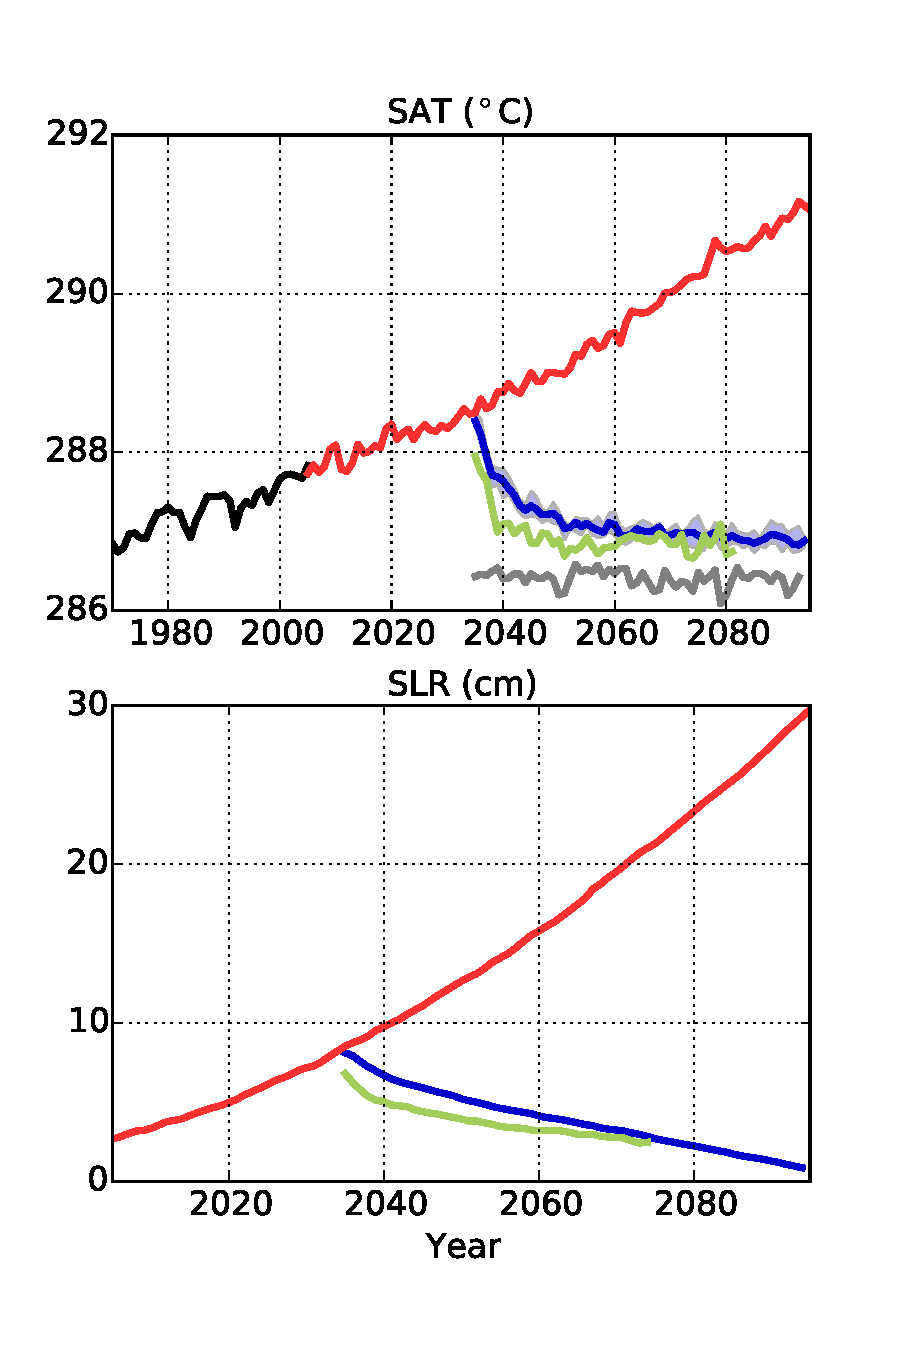
\includegraphics[width=19pc]{figures/SAT_SLR_timeseries_geotimescalesWAISpaper.pdf} %SATSLRtimeseries2.pdf}
\caption{\textbf{Timeseries of SAT and SLR.} Global-mean annual-mean \textbf{(a)} surface air temperature (SAT; $^\circ$C), and \textbf{(b)} steric sea level rise (SLR; cm) due to changes in ocean density, shown as anomalies from 20thC (1970-1999 average). The Sulf curve is an ensemble average. Light blue shading in (a) indicates the spread of the Sulf ensemble of simulations.}
\label{fig:gmts} % @@ do I need to note that years 2076-2078 are interpolated b/c there was missing data?
\end{figure}

\begin{figure}%[htbp] % the star afterwards makes it a one column fig in a 2-col document
%\centering
\noindent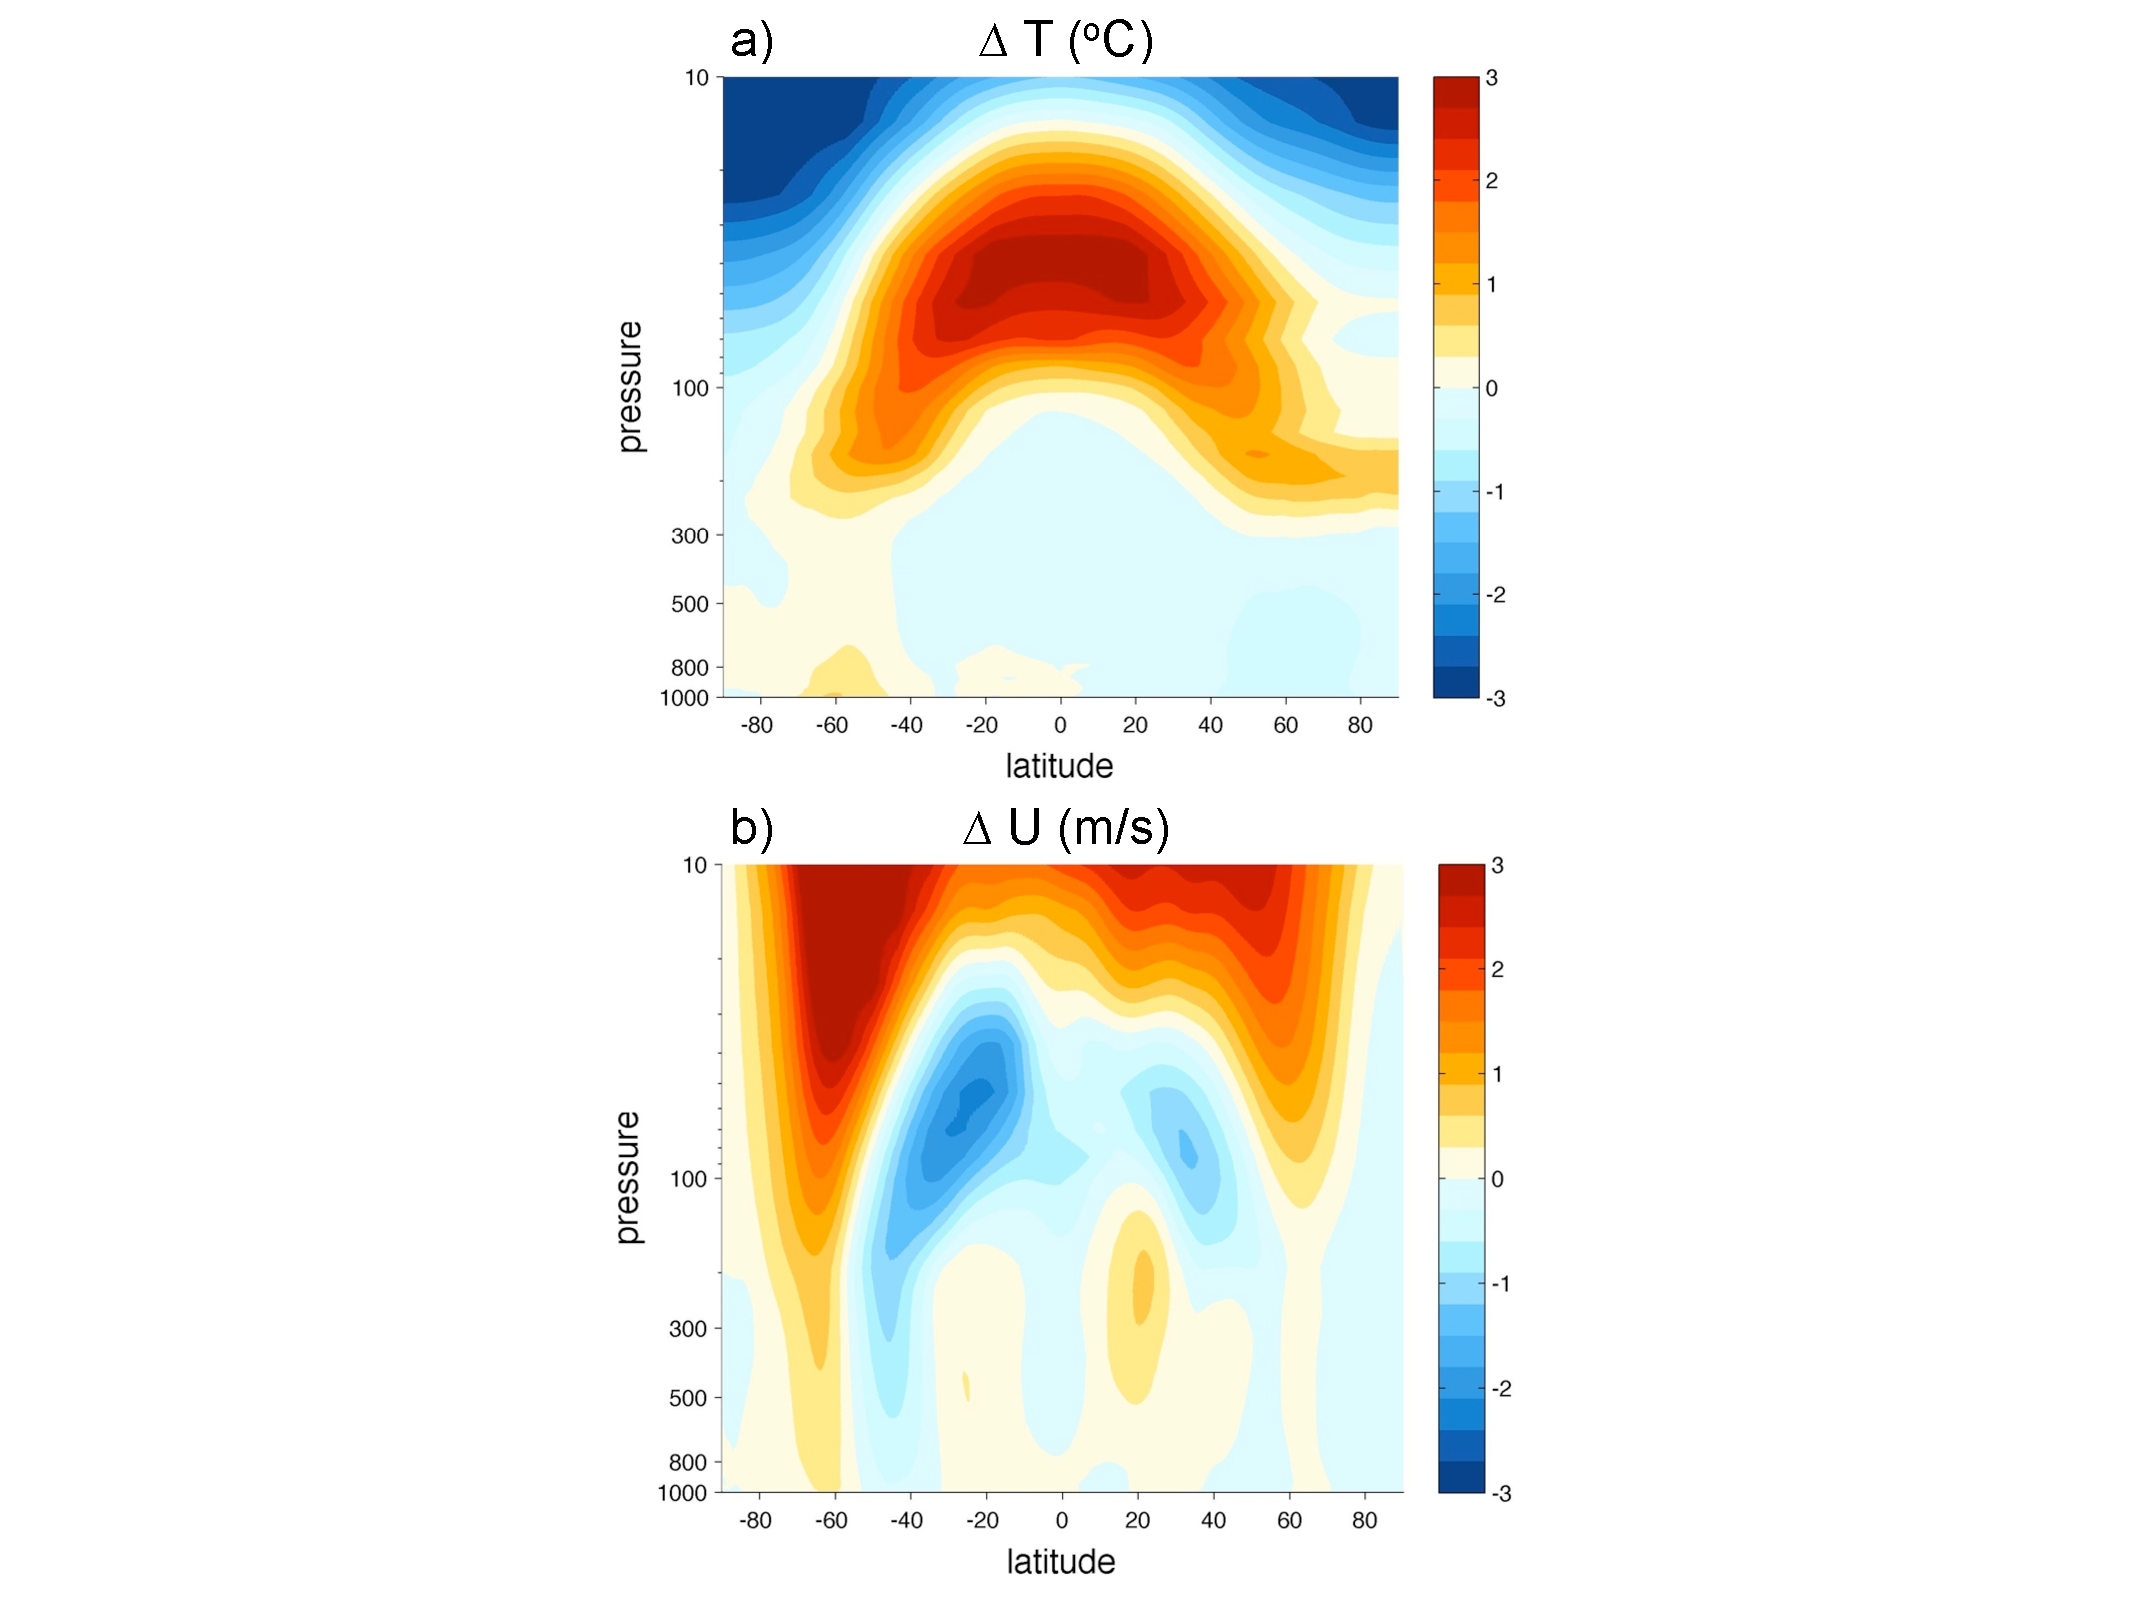
\includegraphics[width=17pc]{figures/verticalU_T_v20thC2.pdf}  % @@  reconfigure to horizontal layout?
\caption{\textbf{Zonal average anomalies with height.} Annual average, zonal average \textbf{(a)} temperature ($^\circ$C) and \textbf{(b)} zonal wind (m/s) averaged from 2045-2054 in the Sulf ensemble minus the 1970-1999 average from 20thC.}
\label{fig:vert}
\end{figure}

\begin{figure}%[htbp] % the star afterwards makes it a one column fig in a 2-col document
%\centering
 \noindent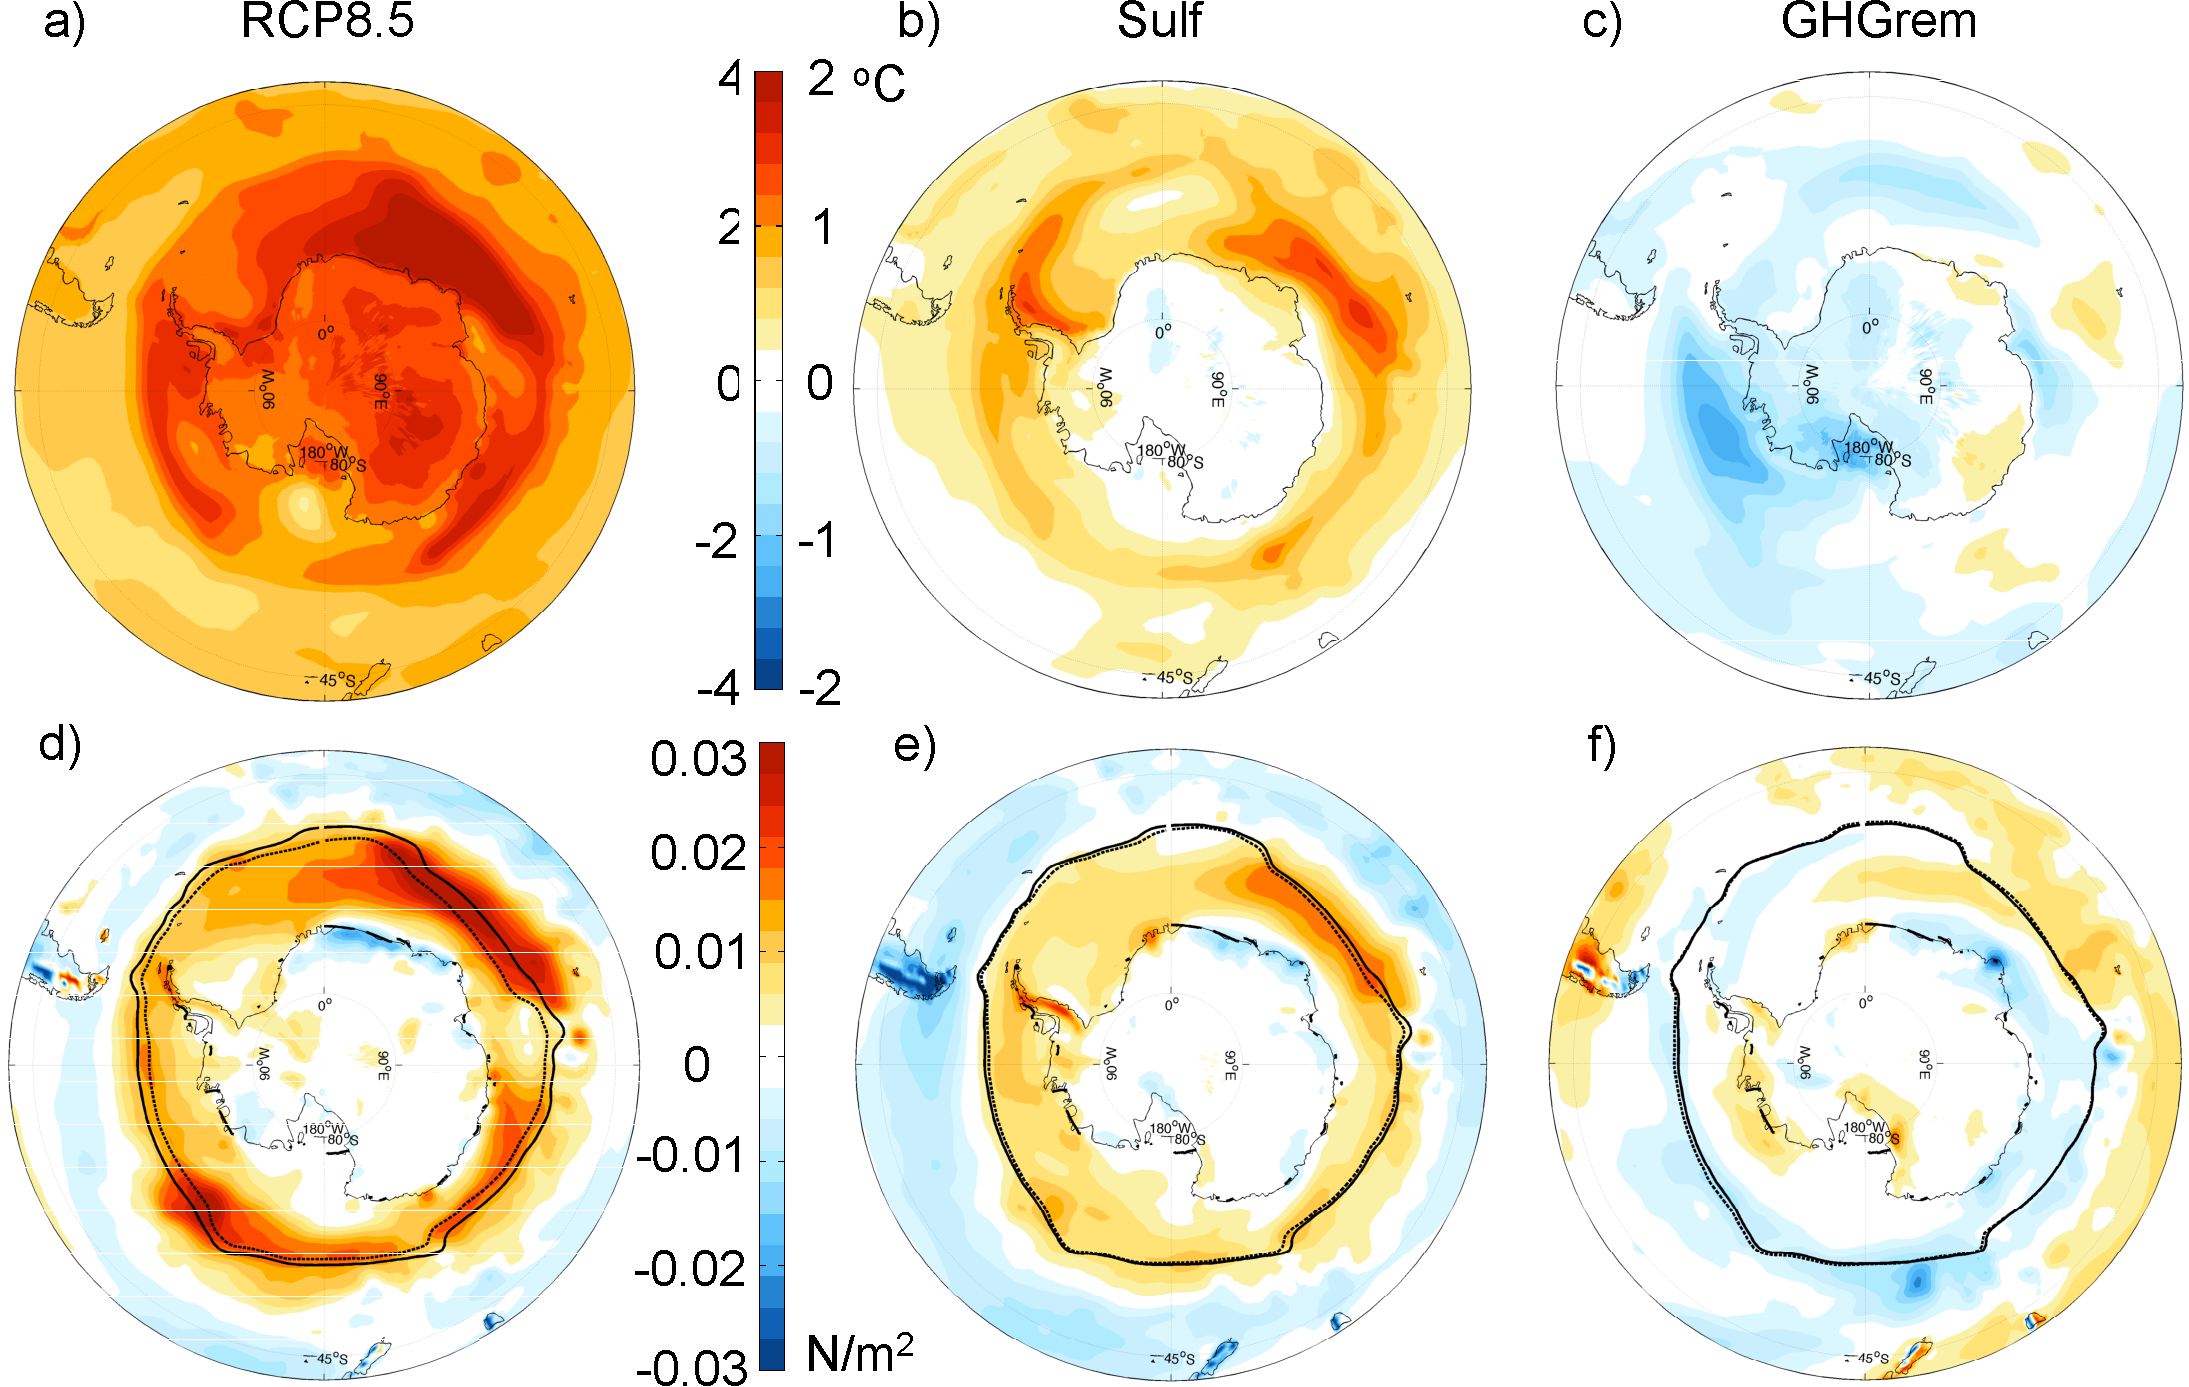
\includegraphics[width=30pc]{figures/SHmaps3.pdf}
\caption{\textbf{SH SAT and zonal wind stress anomaly maps.} Annual mean surface air temperature ($^\circ$C) anomaly from 20thC (1970-1999 mean) for \textbf{(a)} RCP8.5, \textbf{(b)} Sulf, and \textbf{(c)} GHGrem, years 2045-2054. \textbf{(d), (e), and (f)} are as (a), (b), and (c) but for zonal wind stress (N/m$^2$). Positive indicates westerly stress on the ocean. Contours indicate sea ice extent (15\% concentration contour) for the 20thC (solid) and perturbed simulation (dashed).}
\label{fig:shmaps}
\end{figure}

\begin{figure}%[htbp] % the star afterwards makes it a one column fig in a 2-col document
%\centering
 \noindent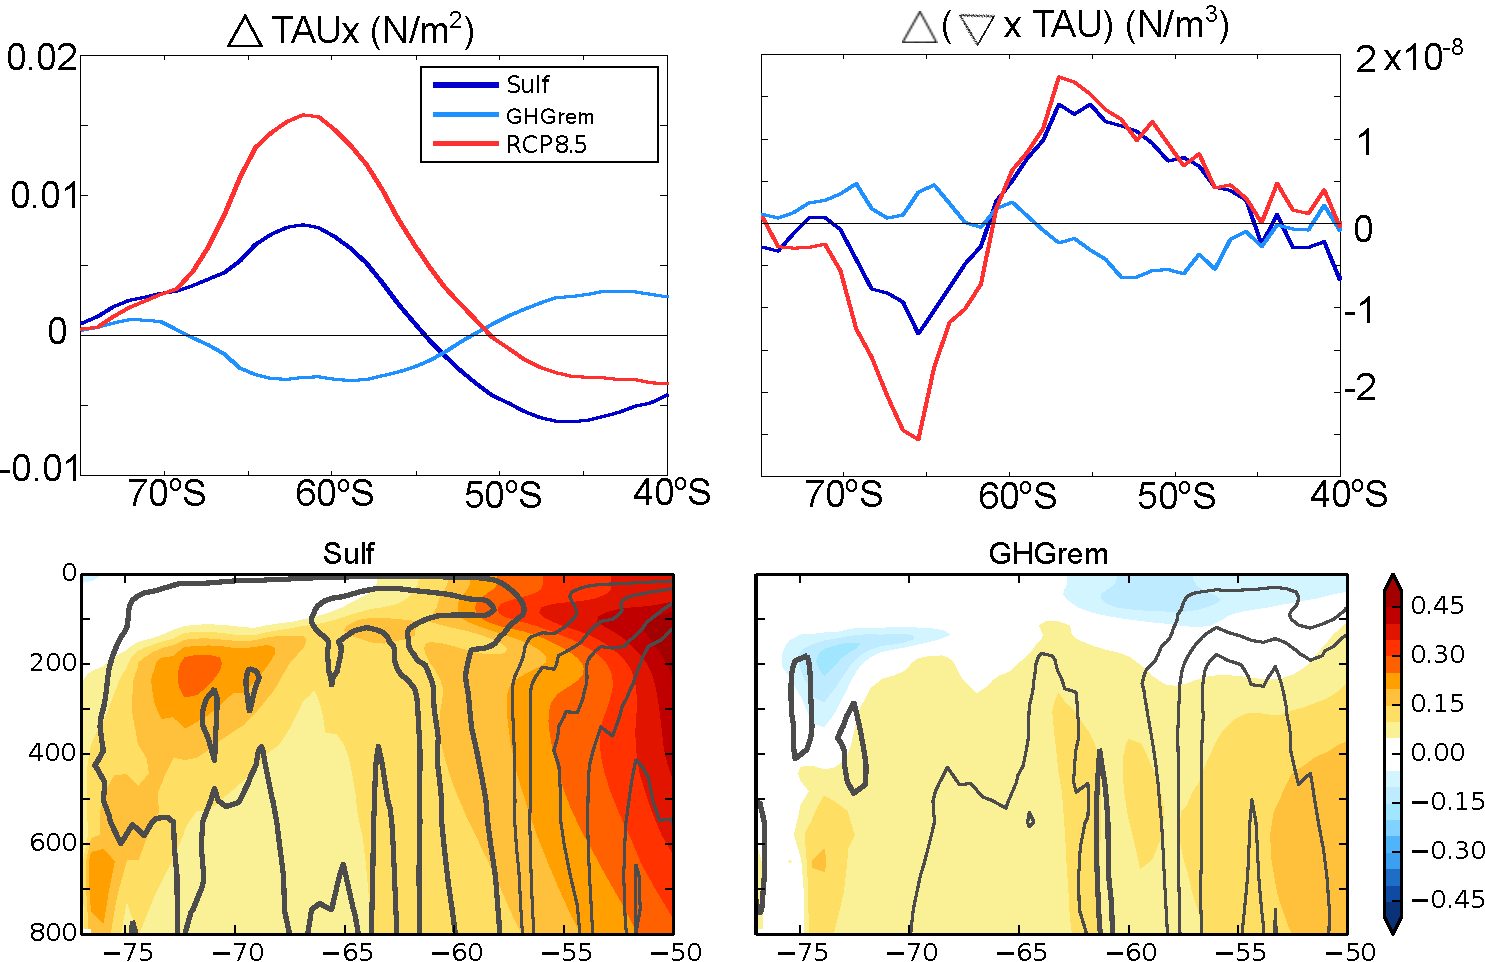
\includegraphics[width=35pc]{figures/TAUcurl_TEMPanomMOCeddy+eul.pdf}
\caption{\textbf{Southern Ocean wind stress, wind stress curl, and potential temperature.} Annual mean, zonal mean \textbf{(a)} zonal wind stress (N/m$^2$) and \textbf{(b)} curl of the wind stress (10$^{-8}$ N/m$^3$) over ocean only, as anomalies from 20thC (1970-1999 mean). Positive indicates westerlies in (a) and downwelling in (b). Annual mean, zonal mean ocean potential temperature ($^\circ$C) anomalies from 20thC with depth for \textbf{(c)} Sulf and \textbf{(d)} GHGrem, years 2045-2054.}
\label{fig:zmtautemp}
\end{figure}

\begin{figure}%[htbp] % the star afterwards makes it a one column fig in a 2-col document
%\centering
 \noindent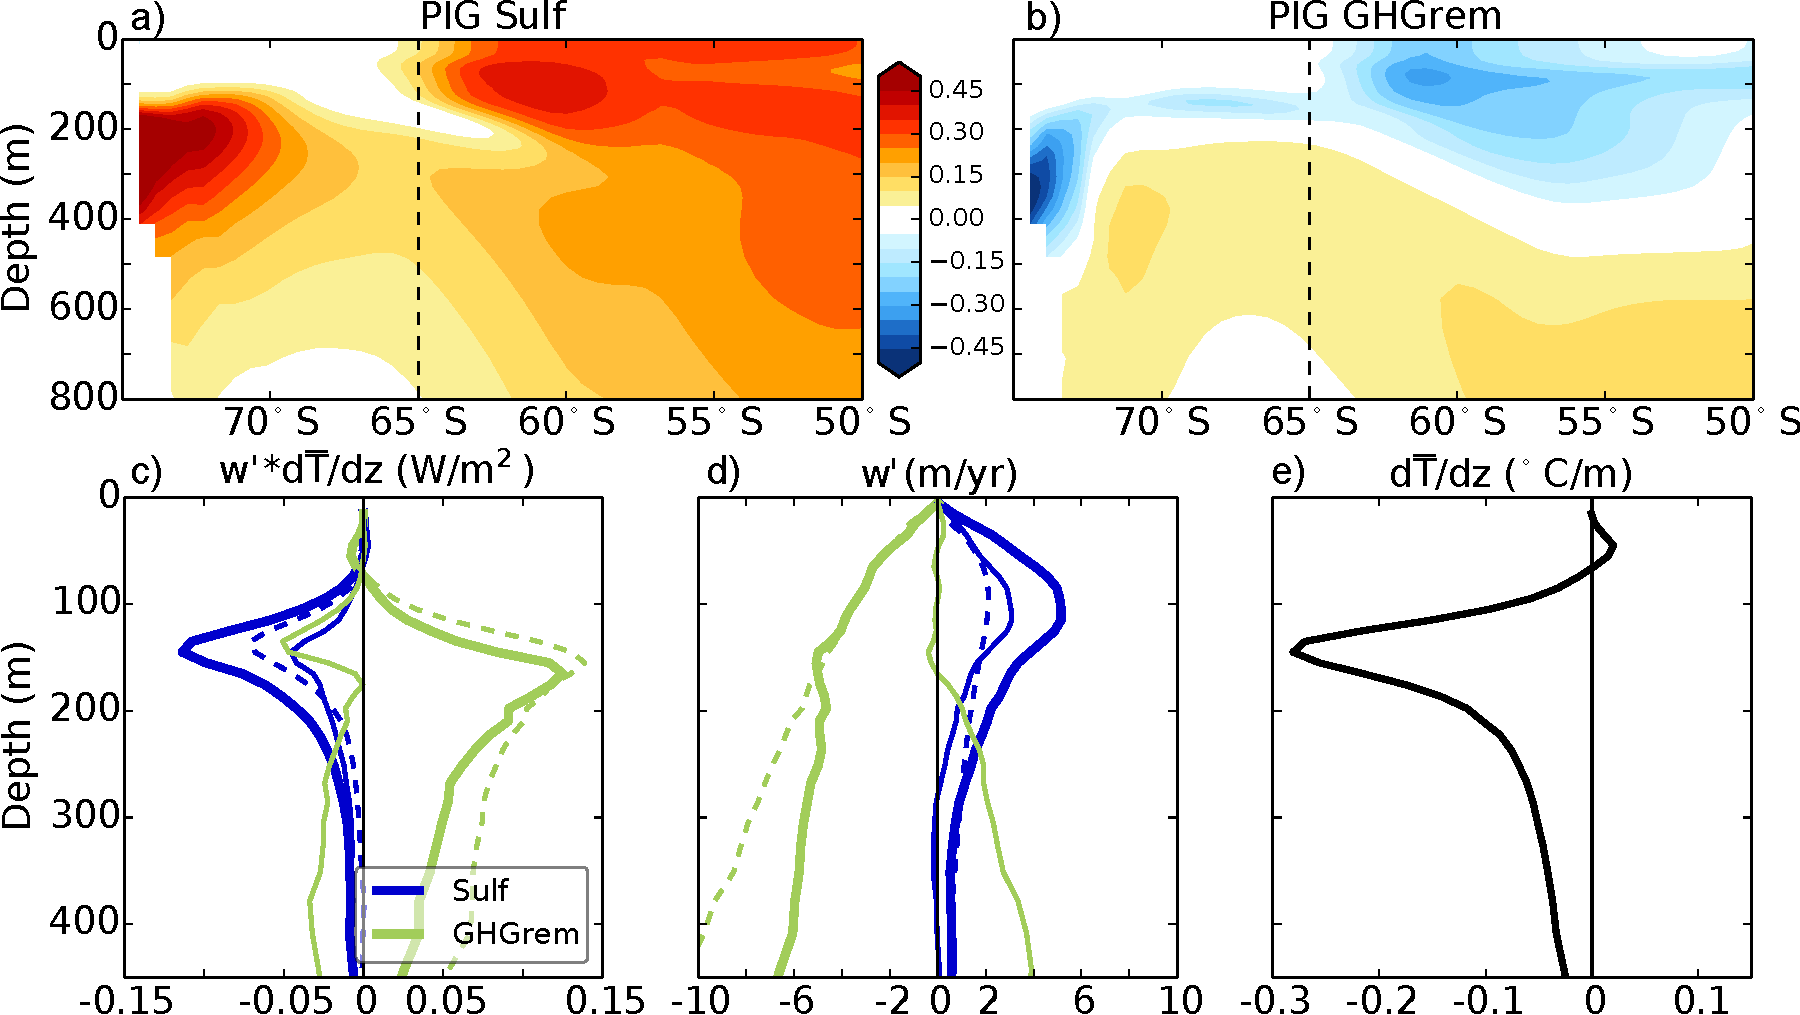
\includegraphics[width=35pc]{figures/TEMPanomvertheat_justPIG.pdf}
\caption{\textbf{PIG region ocean potential temperature and vertical advection tendencies.} Annual mean, zonal mean ocean potential temperature ($^\circ$C) with depth averaged for longitudes 80$^\circ$W to 120$^\circ$W in the Amundsen Sea Embayment / Pine Island Glacier (PIG) region as anomalies from 20thC for \textbf{(a)} Sulf and \textbf{(b)} GHGrem. The vertical dashed line shows the equatorward limit of the region used to calculate the averages shown in panels (c)-(e).\textbf{(c)}  Vertical velocity averaged between 80$^\circ$W-120$^\circ$W and 65$^\circ$S-74$^\circ$S at each depth due to Eulerian (dashed), eddy-induced (thin solid), and total motion (thick solid) as anomalies from 20thC for Sulf (blue) and GHGrem (green) (m/yr). \textbf{(d)} 20thC mean temperature gradient with depth ($^\circ$C/m). Negative indicates increased temperature with increasing depth (z is defined positive up). \textbf{(e)} is as c) but showing vertical advection tendencies (converted to W/m$^2$). Negative values indicate increased vertical advection tendencies.}
\label{fig:pigtemp}
\end{figure}

%%%%%%% supplementary %%%%%%%

%\begin{figure}%[htbp] % the star afterwards makes it a one column fig in a 2-col document
%%\centering
%\noindent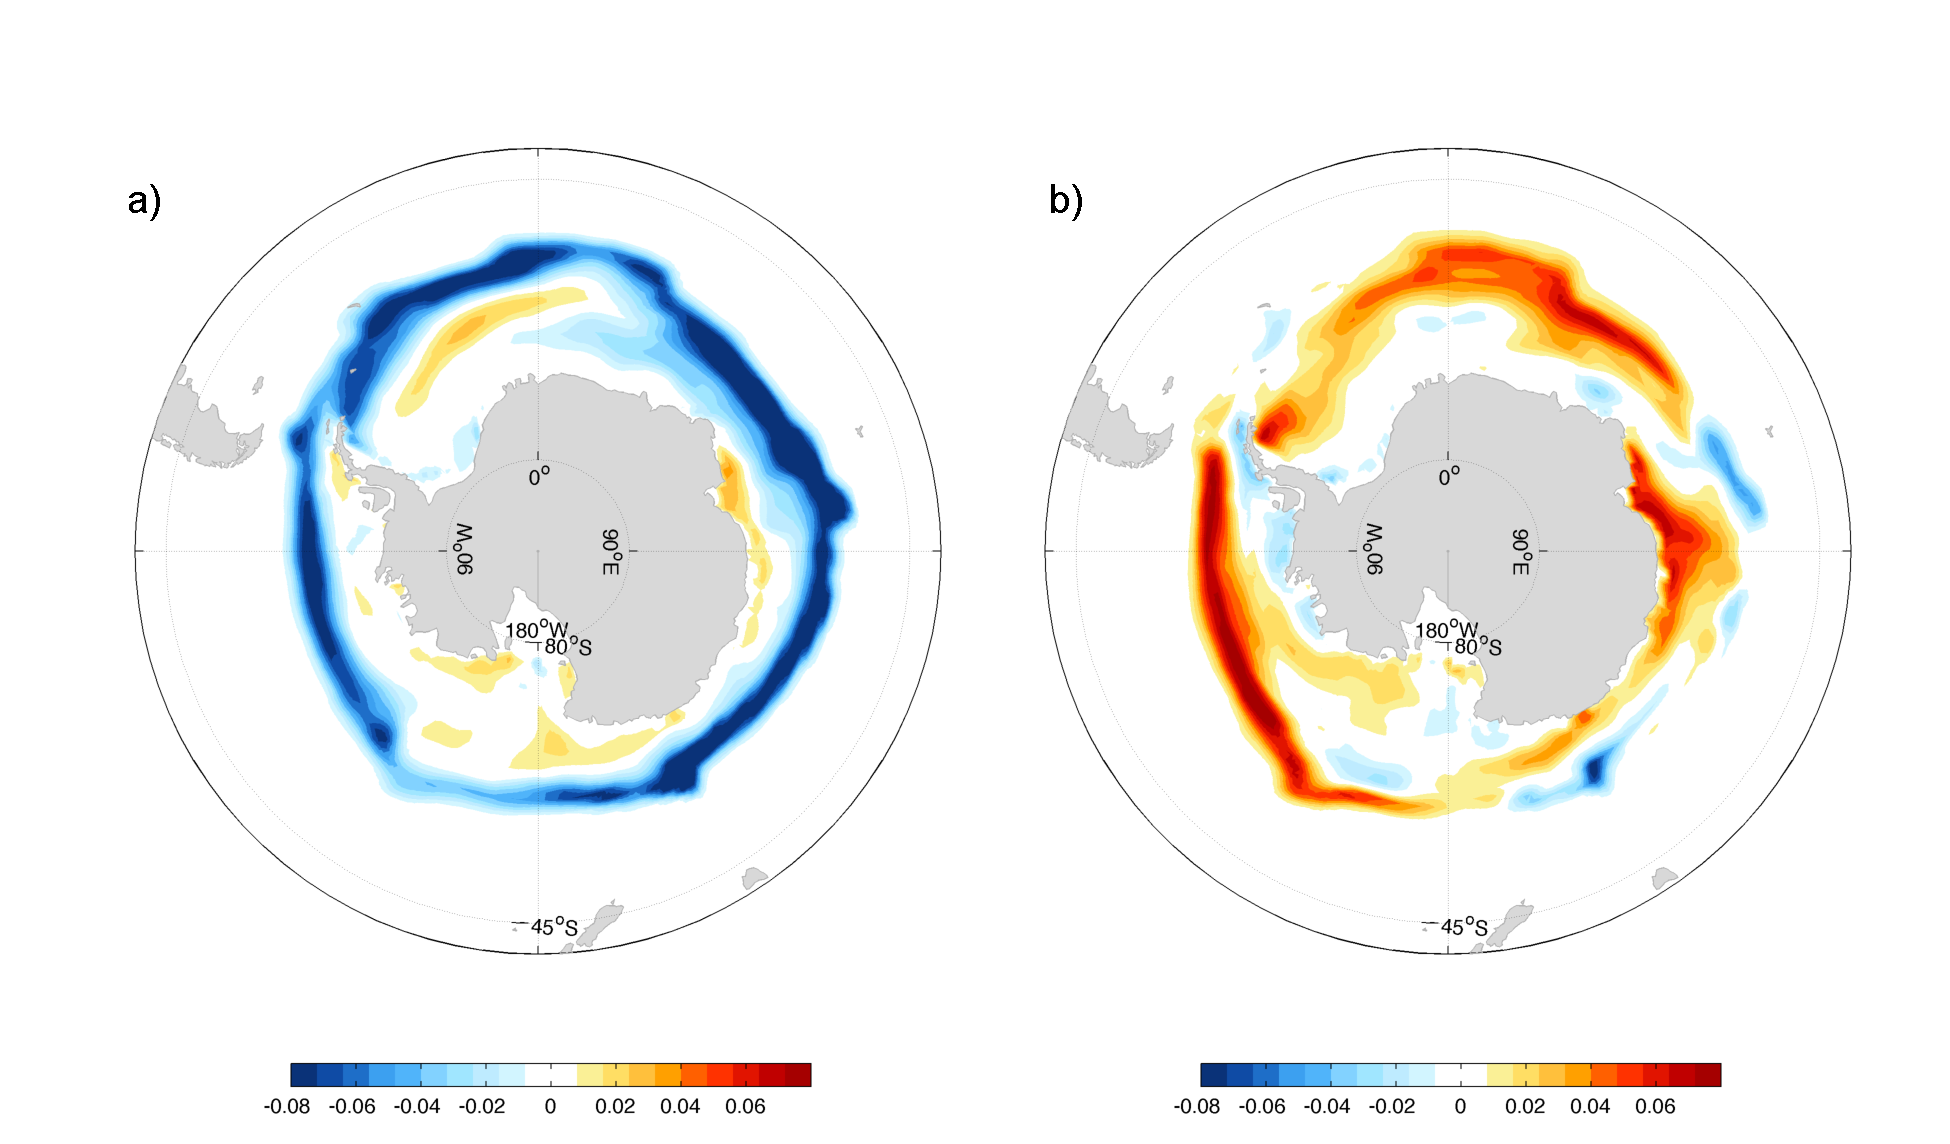
\includegraphics[width=39pc]{figures/SuppFig1.pdf}  % @@  reconfigure to horizontal layout?
%\caption{\textbf{S1: Sea ice concentration anomaly maps.} Annual average sea ice concentration (fraction) anomaly from 20thC (1970-1999 mean) for \textbf{(a)} Sulf and \textbf{(b)} GHGrem, years 2045-2054.}
%\label{fig:supp2}
%\end{figure}
%
%\begin{figure}%[htbp] % the star afterwards makes it a one column fig in a 2-col document
%%\centering
%\noindent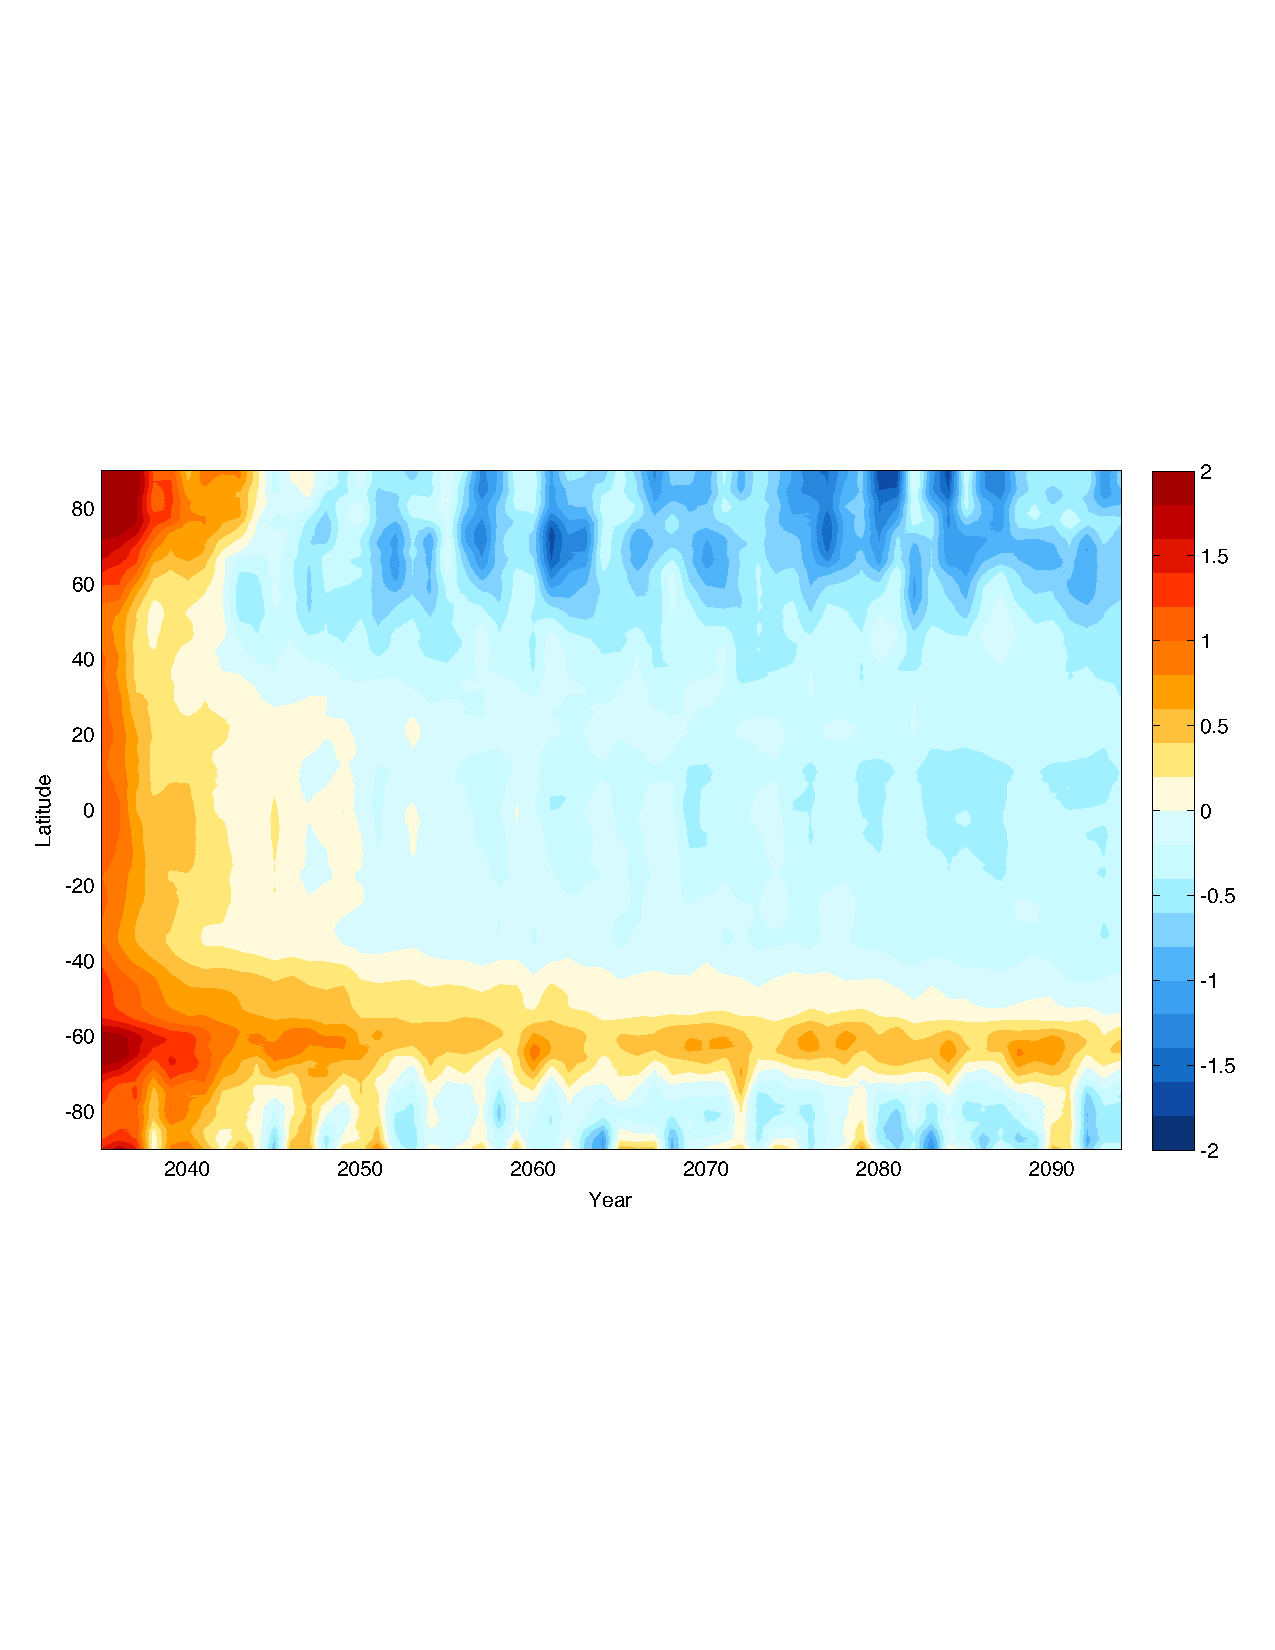
\includegraphics[width=39pc]{figures/SuppFig2.pdf}  % @@  reconfigure to horizontal layout?
%\caption{\textbf{S2: Zonal average SAT anomalies with time.} Annual average, zonal average Sulf surface air temperature ($^\circ$C) with latitude and time as anomalies from the 1970-1999 average from 20thC.}
%\label{fig:supp1}
%\end{figure}
%
%\begin{figure}%[htbp] % the star afterwards makes it a one column fig in a 2-col document
%%\centering
%\noindent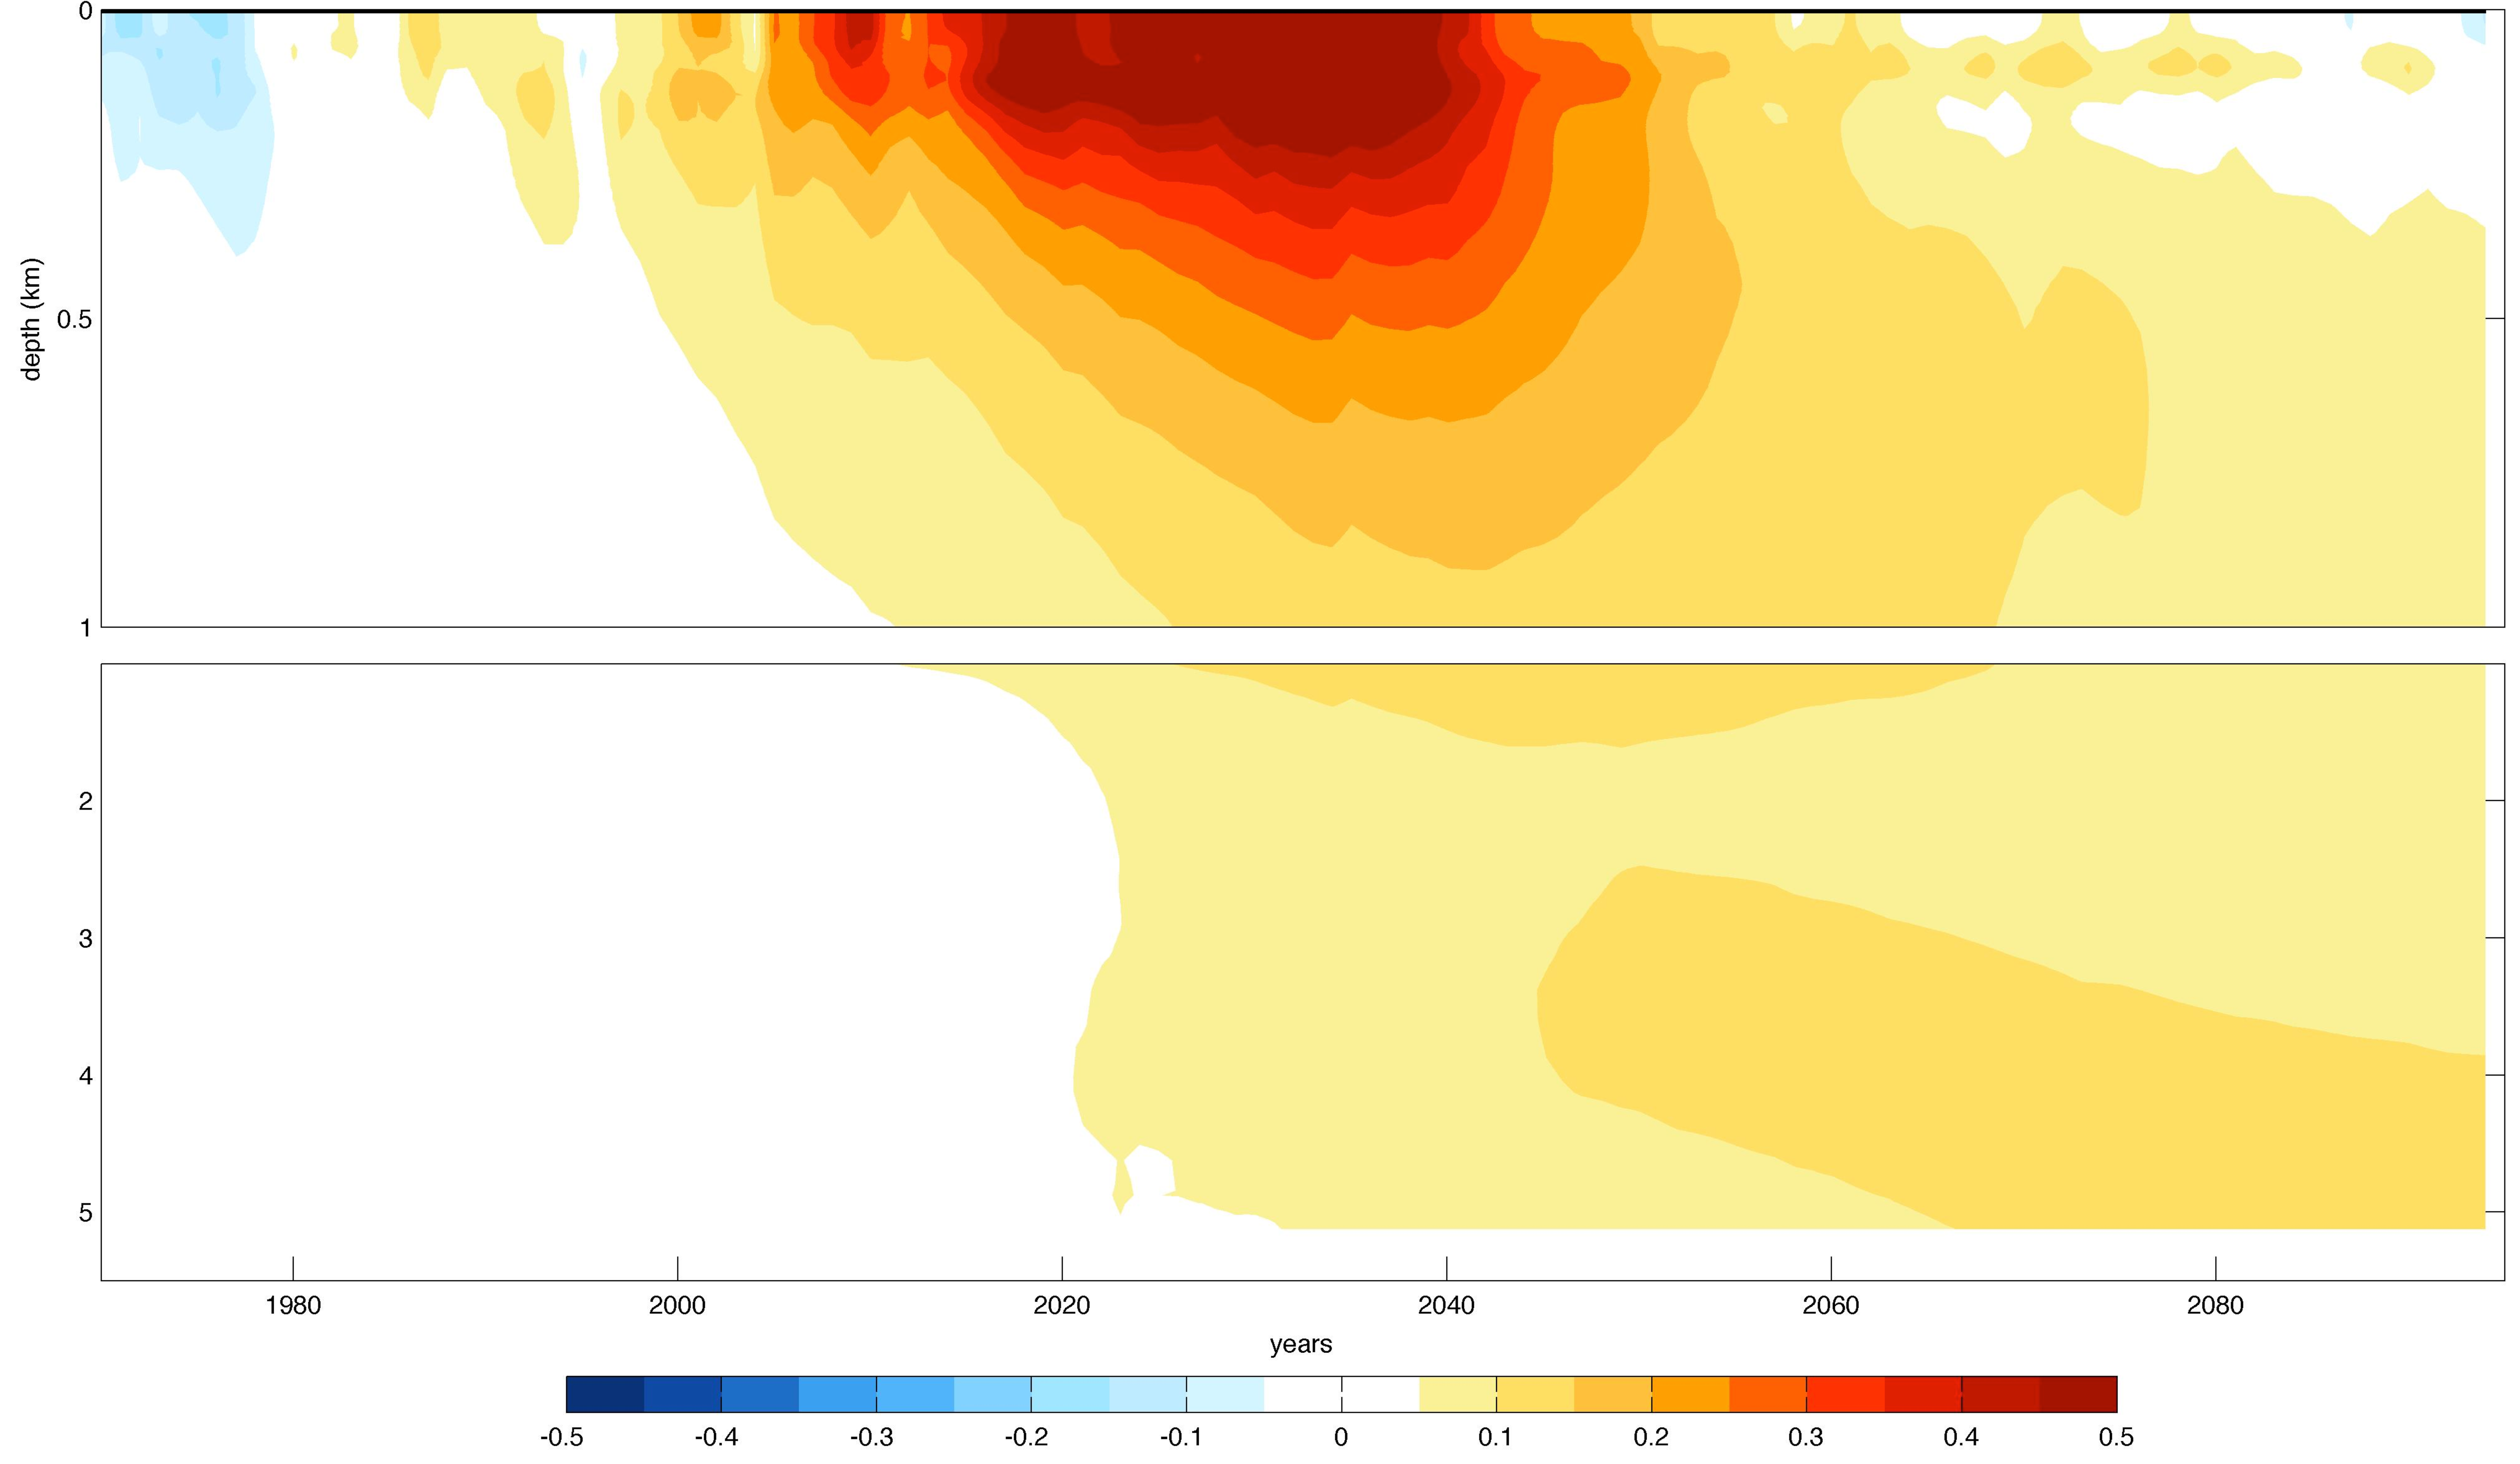
\includegraphics[width=39pc]{figures/SuppFig3.pdf}  % @@  reconfigure to horizontal layout?
%\caption{\textbf{S3: Southern Ocean temperature anomalies with time.} Annual average, Southern Ocean (averaged south of 50$^\circ$S) temperature ($^\circ$C) with depth and time as anomalies from the 1970-1999 average from 20thC. Years 1970-2004 are 20thC anomalies, 2005-2034 are RCP8.5 anomalies, and 2035 to end are Sulf anomalies.}
%\label{fig:supp2}
%\end{figure}



%% Put the bibliography here, most people will use BiBTeX in
%% which case the environment below should be replaced with
%% the \bibliography{} command.

%\begin{thebibliography}{1}
%\end{thebibliography}

\begin{thebibliography}{10}
\expandafter\ifx\csname url\endcsname\relax
  \def\url#1{\texttt{#1}}\fi
\expandafter\ifx\csname urlprefix\endcsname\relax\def\urlprefix{URL }\fi
\providecommand{\bibinfo}[2]{#2}
\providecommand{\eprint}[2][]{\url{#2}}

\bibitem{joughin14}
\bibinfo{author}{Joughin, I.}, \bibinfo{author}{Smith, B.~E.} \&
  \bibinfo{author}{Medley, B.}
\newblock \bibinfo{title}{Marine ice sheet collapse potentially under way for
  the thwaites glacier basin, west antarctica}.
\newblock \emph{\bibinfo{journal}{Science}} \textbf{\bibinfo{volume}{344}},
  \bibinfo{pages}{735--738} (\bibinfo{year}{2014}).
\newblock
  \urlprefix\url{http://www.sciencemag.org/content/344/6185/735.abstract}.
\newblock \eprint{http://www.sciencemag.org/content/344/6185/735.full.pdf}.

\bibitem{rignot14}
\bibinfo{author}{Rignot, E.}, \bibinfo{author}{Mouginot, J.},
  \bibinfo{author}{Morlighem, M.}, \bibinfo{author}{Seroussi, H.} \&
  \bibinfo{author}{Scheuchl, B.}
\newblock \bibinfo{title}{{Widespread, rapid grounding line retreat of Pine
  Island, Thwaites, Smith and Kohler glaciers, West Antarctica from 1992 to
  2011}}.
\newblock \emph{\bibinfo{journal}{Geophysical Research Letters}}
  \textbf{\bibinfo{volume}{41}}, \bibinfo{pages}{3502--3509}
  (\bibinfo{year}{2014}).

\bibitem{favier14}
\bibinfo{author}{Favier, L.} \emph{et~al.}
\newblock \bibinfo{title}{{Retreat of Pine Island Glacier controlled by marine
  ice-sheet instability}}.
\newblock \emph{\bibinfo{journal}{Nature Climate Change}}
  \textbf{\bibinfo{volume}{4}}, \bibinfo{pages}{117--121}
  (\bibinfo{year}{2014}).

\bibitem{church13}
\bibinfo{author}{Church, J.} \emph{et~al.}
\newblock \emph{\bibinfo{title}{Climate Change 2013: The Physical Science
  Basis. Contribution of Working Group I to the Fifth Assessment Report of the
  Intergovernmental Panel on Climate Change}}, chap. \bibinfo{chapter}{Sea
  Level Change} (\bibinfo{publisher}{Cambridge University Press},
  \bibinfo{address}{Cambridge, United Kingdom and New York, NY, USA},
  \bibinfo{year}{2013}).

\bibitem{blackstock09}
\bibinfo{author}{Blackstock, J.~J.} \emph{et~al.}
\newblock \bibinfo{title}{{Climate Engineering Responses to Climate
  Emergencies}}  (\bibinfo{year}{2009}).

\bibitem{joughin11}
\bibinfo{author}{Joughin, I.} \& \bibinfo{author}{Alley, R.~B.}
\newblock \bibinfo{title}{Stability of the west antarctic ice sheet in a
  warming world}.
\newblock \emph{\bibinfo{journal}{Nature Geoscience}}
  \textbf{\bibinfo{volume}{4}}, \bibinfo{pages}{506--513}
  (\bibinfo{year}{2011}).

\bibitem{yin11}
\bibinfo{author}{Yin, J.} \emph{et~al.}
\newblock \bibinfo{title}{Different magnitudes of projected subsurface ocean
  warming around greenland and antarctica}.
\newblock \emph{\bibinfo{journal}{Nature Geosci}} \textbf{\bibinfo{volume}{4}},
  \bibinfo{pages}{524--528} (\bibinfo{year}{2011}).
\newblock \urlprefix\url{http://dx.doi.org/10.1038/ngeo1189}.
\newblock \bibinfo{note}{10.1038/ngeo1189}.

\bibitem{thoma08}
\bibinfo{author}{Thoma, M.}, \bibinfo{author}{Jenkins, A.},
  \bibinfo{author}{Holland, D.} \& \bibinfo{author}{Jacobs, S.}
\newblock \bibinfo{title}{{Modelling Circumpolar Deep Water intrusions on the
  Amundsen Sea continental shelf, Antarctica}}.
\newblock \emph{\bibinfo{journal}{Geophys. Res. Lett.}}
  \textbf{\bibinfo{volume}{35}}, \bibinfo{pages}{L18602}
  (\bibinfo{year}{2008}).
\newblock \bibinfo{note}{Doi:10.1029/2008GL034939}.

\bibitem{oppenheimer98}
\bibinfo{author}{Oppenheimer, M.}
\newblock \bibinfo{title}{{Global warming and the stability of the West
  Antarctic Ice Sheet}}.
\newblock \emph{\bibinfo{journal}{Nature}} \textbf{\bibinfo{volume}{393}},
  \bibinfo{pages}{325--332} (\bibinfo{year}{1998}).
\newblock \bibinfo{note}{10.1038/30661}.

\bibitem{pritchard12}
\bibinfo{author}{Pritchard, H.~D.} \emph{et~al.}
\newblock \bibinfo{title}{Antarctic ice-sheet loss driven by basal melting of
  ice shelves}.
\newblock \emph{\bibinfo{journal}{Nature}} \textbf{\bibinfo{volume}{484}},
  \bibinfo{pages}{502--505} (\bibinfo{year}{2012}).

\bibitem{moore10}
\bibinfo{author}{Moore, J.~C.}, \bibinfo{author}{Jevrejeva, S.} \&
  \bibinfo{author}{Grinsted, A.}
\newblock \bibinfo{title}{Efficacy of geoengineering to limit 21st century
  sea-level rise}.
\newblock \emph{\bibinfo{journal}{Proceedings of the National Academy of
  Sciences}}  (\bibinfo{year}{2010}).

\bibitem{church05}
\bibinfo{author}{Church, J.~A.}, \bibinfo{author}{White, N.~J.} \&
  \bibinfo{author}{Arblaster, J.~M.}
\newblock \bibinfo{title}{Significant decadal-scale impact of volcanic
  eruptions on sea level and ocean heat content}.
\newblock \emph{\bibinfo{journal}{Nature}} \textbf{\bibinfo{volume}{438}},
  \bibinfo{pages}{74--77} (\bibinfo{year}{2005}).
\newblock \bibinfo{note}{10.1038/nature04237}.

\bibitem{gleckler06}
\bibinfo{author}{Gleckler, P.~J.} \emph{et~al.}
\newblock \bibinfo{title}{Krakatoa lives: The effect of volcanic eruptions on
  ocean heat content and thermal expansion}.
\newblock \emph{\bibinfo{journal}{Geophys. Res. Lett.}}
  \textbf{\bibinfo{volume}{33}}, \bibinfo{pages}{L17702}
  (\bibinfo{year}{2006}).

\bibitem{irvine12}
\bibinfo{author}{Irvine, P.~J.}, \bibinfo{author}{Sriver, R.~L.} \&
  \bibinfo{author}{Keller, K.}
\newblock \bibinfo{title}{Tension between reducing sea-level rise and global
  warming through solar-radiation management}.
\newblock \emph{\bibinfo{journal}{Nature Climate Change}}
  \textbf{\bibinfo{volume}{2}}, \bibinfo{pages}{97--100}
  (\bibinfo{year}{2012}).

\bibitem{steig13}
\bibinfo{author}{Steig, E.~J.} \emph{et~al.}
\newblock \bibinfo{title}{Recent climate and ice-sheet changes in west
  antarctica compared with the past 2,000 years}.
\newblock \emph{\bibinfo{journal}{Nature Geosci}} \textbf{\bibinfo{volume}{6}},
  \bibinfo{pages}{372--375} (\bibinfo{year}{2013}).
\newblock \urlprefix\url{http://dx.doi.org/10.1038/ngeo1778}.

\bibitem{fyfe07}
\bibinfo{author}{Fyfe, J.~C.}, \bibinfo{author}{Saenko, O.~A.},
  \bibinfo{author}{Zickfeld, K.}, \bibinfo{author}{Eby, M.} \&
  \bibinfo{author}{Weaver, A.~J.}
\newblock \bibinfo{title}{{The Role of Poleward-Intensifying Winds on Southern
  Ocean Warming}}.
\newblock \emph{\bibinfo{journal}{Journal of Climate}}
  \textbf{\bibinfo{volume}{20}}, \bibinfo{pages}{5391--5400}
  (\bibinfo{year}{2007}).

\bibitem{spence14}
\bibinfo{author}{Spence, P.} \emph{et~al.}
\newblock \bibinfo{title}{Rapid subsurface warming and circulation changes of
  antarctic coastal waters by poleward shifting winds}.
\newblock \emph{\bibinfo{journal}{Geophysical Research Letters}}
  \textbf{\bibinfo{volume}{41}}, \bibinfo{pages}{4601--4610}
  (\bibinfo{year}{2014}).
\newblock \urlprefix\url{http://dx.doi.org/10.1002/2014GL060613}.

\bibitem{notz09}
\bibinfo{author}{Notz, D.}
\newblock \bibinfo{title}{{The future of ice sheets and sea ice: Between
  reversible retreat and unstoppable loss}}.
\newblock \emph{\bibinfo{journal}{Proceedings of the National Academy of
  Sciences}} \textbf{\bibinfo{volume}{106}}, \bibinfo{pages}{20590--20595}
  (\bibinfo{year}{2009}).

\bibitem{gillett11}
\bibinfo{author}{Gillett, N.~P.}, \bibinfo{author}{Arora, V.~K.},
  \bibinfo{author}{Zickfeld, K.}, \bibinfo{author}{Marshall, S.~J.} \&
  \bibinfo{author}{Merryfield, W.~J.}
\newblock \bibinfo{title}{Ongoing climate change following a complete cessation
  of carbon dioxide emissions}.
\newblock \emph{\bibinfo{journal}{Nature Geosci}} \textbf{\bibinfo{volume}{4}},
  \bibinfo{pages}{83--87} (\bibinfo{year}{2011}).
\newblock \bibinfo{note}{10.1038/ngeo1047}.

\bibitem{ammann10}
\bibinfo{author}{Ammann, C.~M.}, \bibinfo{author}{Washington, W.~M.},
  \bibinfo{author}{Meehl, G.~A.}, \bibinfo{author}{Buja, L.} \&
  \bibinfo{author}{Teng, H.}
\newblock \bibinfo{title}{Climate engineering through artificial enhancement of
  natural forcings: Magnitudes and implied consequences}.
\newblock \emph{\bibinfo{journal}{J. Geophys. Res.}}
  \textbf{\bibinfo{volume}{115}}, \bibinfo{pages}{D22109}
  (\bibinfo{year}{2010}).
\newblock \bibinfo{note}{Doi:10.1029/2009JD012878}.

\bibitem{mccusker12}
\bibinfo{author}{McCusker, K.~E.}, \bibinfo{author}{Battisti, D.~S.} \&
  \bibinfo{author}{Bitz, C.~M.}
\newblock \bibinfo{title}{The climate response to stratospheric sulfate
  injections and implications for addressing climate emergencies}.
\newblock \emph{\bibinfo{journal}{Journal of Climate}}
  \textbf{\bibinfo{volume}{25}}, \bibinfo{pages}{3096--3116}
  (\bibinfo{year}{2012}).
\newblock \bibinfo{note}{Doi:http://dx.doi.org/10.1175/JCLI-D-11-00183.1}.

\bibitem{gillett03}
\bibinfo{author}{Gillett, N.~P.} \& \bibinfo{author}{Thompson, D. W.~J.}
\newblock \bibinfo{title}{Simulation of recent southern hemisphere climate
  change}.
\newblock \emph{\bibinfo{journal}{Science}} \textbf{\bibinfo{volume}{302}},
  \bibinfo{pages}{273--275} (\bibinfo{year}{2003}).
\newblock
  \urlprefix\url{http://www.sciencemag.org/content/302/5643/273.abstract}.

\bibitem{gillett13}
\bibinfo{author}{Gillett, N.~P.}, \bibinfo{author}{Fyfe, J.~C.} \&
  \bibinfo{author}{Parker, D.~E.}
\newblock \bibinfo{title}{Attribution of observed sea level pressure trends to
  greenhouse gas, aerosol and ozone changes}.
\newblock \emph{\bibinfo{journal}{Geophys. Res. Lett. Geophysical Research
  Letters}}  (\bibinfo{year}{2013}).

\bibitem{sigmond11}
\bibinfo{author}{Sigmond, M.}, \bibinfo{author}{Reader, M.},
  \bibinfo{author}{Fyfe, J.} \& \bibinfo{author}{Gillett, N.}
\newblock \bibinfo{title}{Drivers of past and future southern ocean change:
  Stratospheric ozone versus greenhouse gas impacts}.
\newblock \emph{\bibinfo{journal}{Geophysical Research Letters}}
  \textbf{\bibinfo{volume}{38}}, \bibinfo{pages}{L12601}
  (\bibinfo{year}{2011}).

\bibitem{thompson11}
\bibinfo{author}{Thompson, D.~W.} \emph{et~al.}
\newblock \bibinfo{title}{Signatures of the antarctic ozone hole in southern
  hemisphere surface climate change}.
\newblock \emph{\bibinfo{journal}{Nature Geoscience}}
  \textbf{\bibinfo{volume}{4}}, \bibinfo{pages}{741--749}
  (\bibinfo{year}{2011}).

\bibitem{polvani11}
\bibinfo{author}{Polvani~L.M, P. M. D.~C.}
\newblock \bibinfo{title}{Large cancellation, due to ozone recovery, of future
  southern hemisphere atmospheric circulation trends}.
\newblock \emph{\bibinfo{journal}{Geophys. Res. Lett. Geophysical Research
  Letters}} \textbf{\bibinfo{volume}{38}} (\bibinfo{year}{2011}).

\bibitem{chen07}
\bibinfo{author}{Chen, G.} \& \bibinfo{author}{Held, I.~M.}
\newblock \bibinfo{title}{Phase speed spectra and the recent poleward shift of
  southern hemisphere surface westerlies}.
\newblock \emph{\bibinfo{journal}{Geophysical Research Letters}}
  \textbf{\bibinfo{volume}{34}}, \bibinfo{pages}{L21805}
  (\bibinfo{year}{2007}).
\newblock \urlprefix\url{http://dx.doi.org/10.1029/2007GL031200}.

\bibitem{ferraro11}
\bibinfo{author}{Ferraro, A.~J.}, \bibinfo{author}{Highwood, E.~J.} \&
  \bibinfo{author}{Charlton-Perez, A.~J.}
\newblock \bibinfo{title}{Stratospheric heating by potential geoengineering
  aerosols}.
\newblock \emph{\bibinfo{journal}{Geophysical Research Letters}}
  \textbf{\bibinfo{volume}{38}}, \bibinfo{pages}{L24706}
  (\bibinfo{year}{2011}).
\newblock \urlprefix\url{http://dx.doi.org/10.1029/2011GL049761}.

\bibitem{rignot02}
\bibinfo{author}{Rignot, E.} \& \bibinfo{author}{Jacobs, S.~S.}
\newblock \bibinfo{title}{Rapid bottom melting widespread near antarctic ice
  sheet grounding lines}.
\newblock \emph{\bibinfo{journal}{Science}} \textbf{\bibinfo{volume}{296}},
  \bibinfo{pages}{2020--2023} (\bibinfo{year}{2002}).

\bibitem{shepherd12}
\bibinfo{author}{Shepherd, A. e.~a.}
\newblock \bibinfo{title}{{A Reconciled Estimate of Ice-Sheet Mass Balance}}.
\newblock \emph{\bibinfo{journal}{Science}} \textbf{\bibinfo{volume}{338}},
  \bibinfo{pages}{1183--1189} (\bibinfo{year}{2012}).

\bibitem{robock08c}
\bibinfo{author}{Robock, A.}
\newblock \bibinfo{title}{20 reasons why geoengineering may be a bad idea}.
\newblock \emph{\bibinfo{journal}{Bulletin of the Atomic Scientists}}
  (\bibinfo{year}{2008c}).

\bibitem{tilmes08}
\bibinfo{author}{Tilmes, S.}, \bibinfo{author}{Muller, R.} \&
  \bibinfo{author}{Salawitch, R.}
\newblock \bibinfo{title}{{The Sensitivity of Polar Ozone Depletion to Proposed
  Geoengineering Schemes}}.
\newblock \emph{\bibinfo{journal}{Science}} \textbf{\bibinfo{volume}{320}},
  \bibinfo{pages}{1201--1204} (\bibinfo{year}{2008}).

\bibitem{heckendorn09}
\bibinfo{author}{Heckendorn, P.} \emph{et~al.}
\newblock \bibinfo{title}{{The impact of geoengineering aerosols on
  stratospheric temperature and ozone}}.
\newblock \emph{\bibinfo{journal}{Environmental Research Letters}}
  \textbf{\bibinfo{volume}{4}}, \bibinfo{pages}{045108} (\bibinfo{year}{2009}).

\bibitem{jones13}
\bibinfo{author}{Jones, A.} \emph{et~al.}
\newblock \bibinfo{title}{The impact of abrupt suspension of solar radiation
  management (termination effect) in experiment g2 of the geoengineering model
  intercomparison project (geomip)}.
\newblock \emph{\bibinfo{journal}{Journal of Geophysical Research:
  Atmospheres}} \textbf{\bibinfo{volume}{118}} (\bibinfo{year}{2013}).

\bibitem{mccusker14}
\bibinfo{author}{McCusker, K.~E.}, \bibinfo{author}{Armour, K.~C.},
  \bibinfo{author}{Bitz, C.~M.} \& \bibinfo{author}{Battisti, D.~S.}
\newblock \bibinfo{title}{Rapid and extensive warming following cessation of
  solar radiation management}.
\newblock \emph{\bibinfo{journal}{Environmental Research Letters}}
  \textbf{\bibinfo{volume}{9}}, \bibinfo{pages}{024005} (\bibinfo{year}{2014}).
\newblock \urlprefix\url{http://stacks.iop.org/1748-9326/9/i=2/a=024005}.

\bibitem{feely04}
\bibinfo{author}{Feely, R.~A.} \emph{et~al.}
\newblock \bibinfo{title}{Impact of anthropogenic co$_2$ on the caco3 system in
  the oceans}.
\newblock \emph{\bibinfo{journal}{Science}} \textbf{\bibinfo{volume}{305}},
  \bibinfo{pages}{362--366} (\bibinfo{year}{2004}).
\newblock
  \urlprefix\url{http://www.sciencemag.org/content/305/5682/362.abstract}.

\bibitem{bala08}
\bibinfo{author}{Bala, G.}, \bibinfo{author}{Duffy, P.~B.} \&
  \bibinfo{author}{Taylor, K.~E.}
\newblock \bibinfo{title}{{Impact of geoengineering schemes on the global
  hydrological cycle}}.
\newblock \emph{\bibinfo{journal}{Proceedings of the National Academy of
  Sciences}} \textbf{\bibinfo{volume}{105}}, \bibinfo{pages}{7664--7669}
  (\bibinfo{year}{2008}).

\bibitem{gent11}
\bibinfo{author}{Gent, P.~R.} \emph{et~al.}
\newblock \bibinfo{title}{The community climate system model version 4}.
\newblock \emph{\bibinfo{journal}{Journal of Climate}}
  \textbf{\bibinfo{volume}{24}}, \bibinfo{pages}{4973--4991}
  (\bibinfo{year}{2011}).

\end{thebibliography}


%\bibliographystyle{ametsoc}
%\bibliography{allrefs}





% ~/bibtexrefs/allrefs  == this is version controlled now, but will have to just copy into current dir?


%% Here is the endmatter stuff: Supplementary Info, etc.
%% Use \item's to separate, default label is "Acknowledgements"

\begin{addendum}
\item[Acknowledgements] We thank Judy Twedt for helpful discussion on experiment design and analysis and Dr. Colin Goldblatt for comments that improved the manuscript. This research was funded by the Tamaki Foundation and supported in part by the National Science Foundation through TeraGrid resources provided by the Texas Advanced Computing Center under Grant TG-ATM090059.
\item[Author Contributions] 
 \item[Competing Interests] The authors declare that they have no competing financial interests.
\item[Correspondence] Correspondence and requests for materials should be addressed to K.E.M.~(email: kemccusk@uvic.ca).
\end{addendum}

%%
%% TABLES
%%
%% If there are any tables, put them here.
%%

\end{document}
